

%\setcounter{chapter}{33}
\chapter{Classification, Localization and Segmentation of Objects}
\label{chapter:object_recognition}

%\reviewcomment{References missing.}


%why we need a learning based system?

%Output representation (this can  just  be a figure): this addresses the question of how is the output specified (a label, a bounding box, a 3D model, ...).

\section{Introduction}

There are many tasks that researchers use to address  the problem of recognition. Although  the ultimate goal is to tell what something it is by looking at it, the way that you will answer the question will change the approach that you will use. For instance, you could say, ``That is a chair'' and just point at it, or we could ask you to indicate all of the visible parts of the chair, which might be a lot harder if the chair is partially occluded by other chairs producing a sea of legs. It can be hard to precisely delineate the chair if we cannot tell which legs belong to it. In other cases, identifying what a chair is might be difficult, requiring understanding of its context and social conventions.  

  
\begin{figure}[h]
\centerline{
%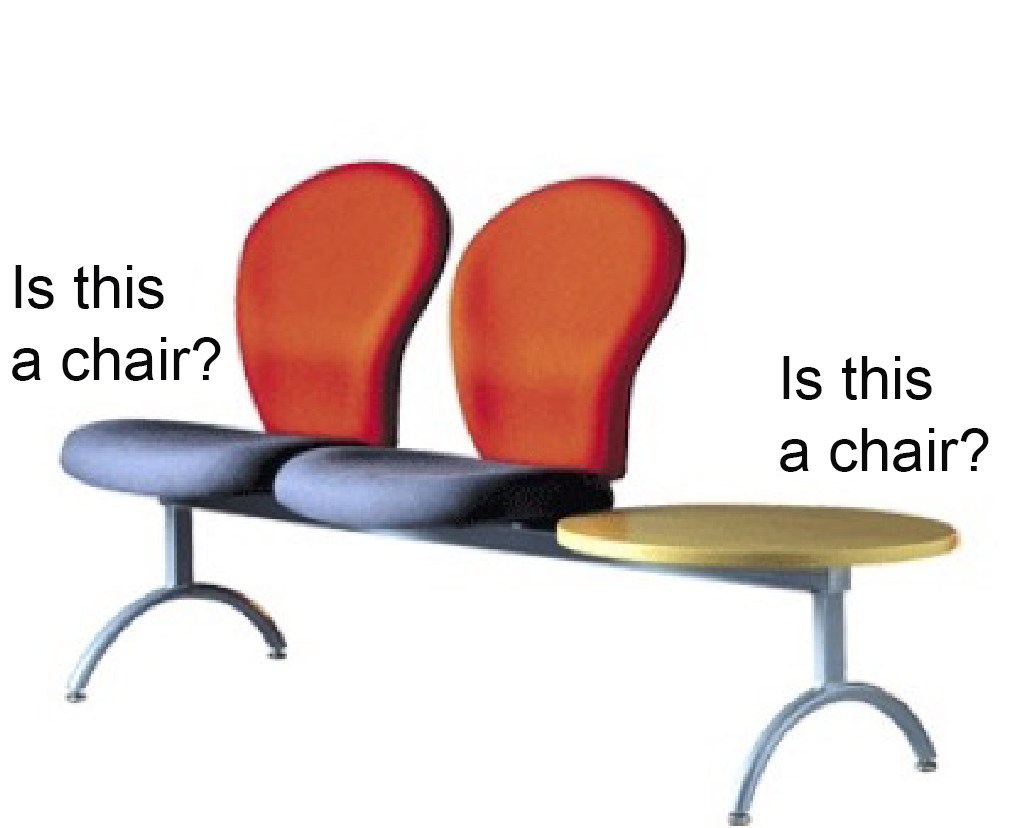
\includegraphics[width=0.4\linewidth]{figures/object_recognition/chair_or_table_text.jpg}
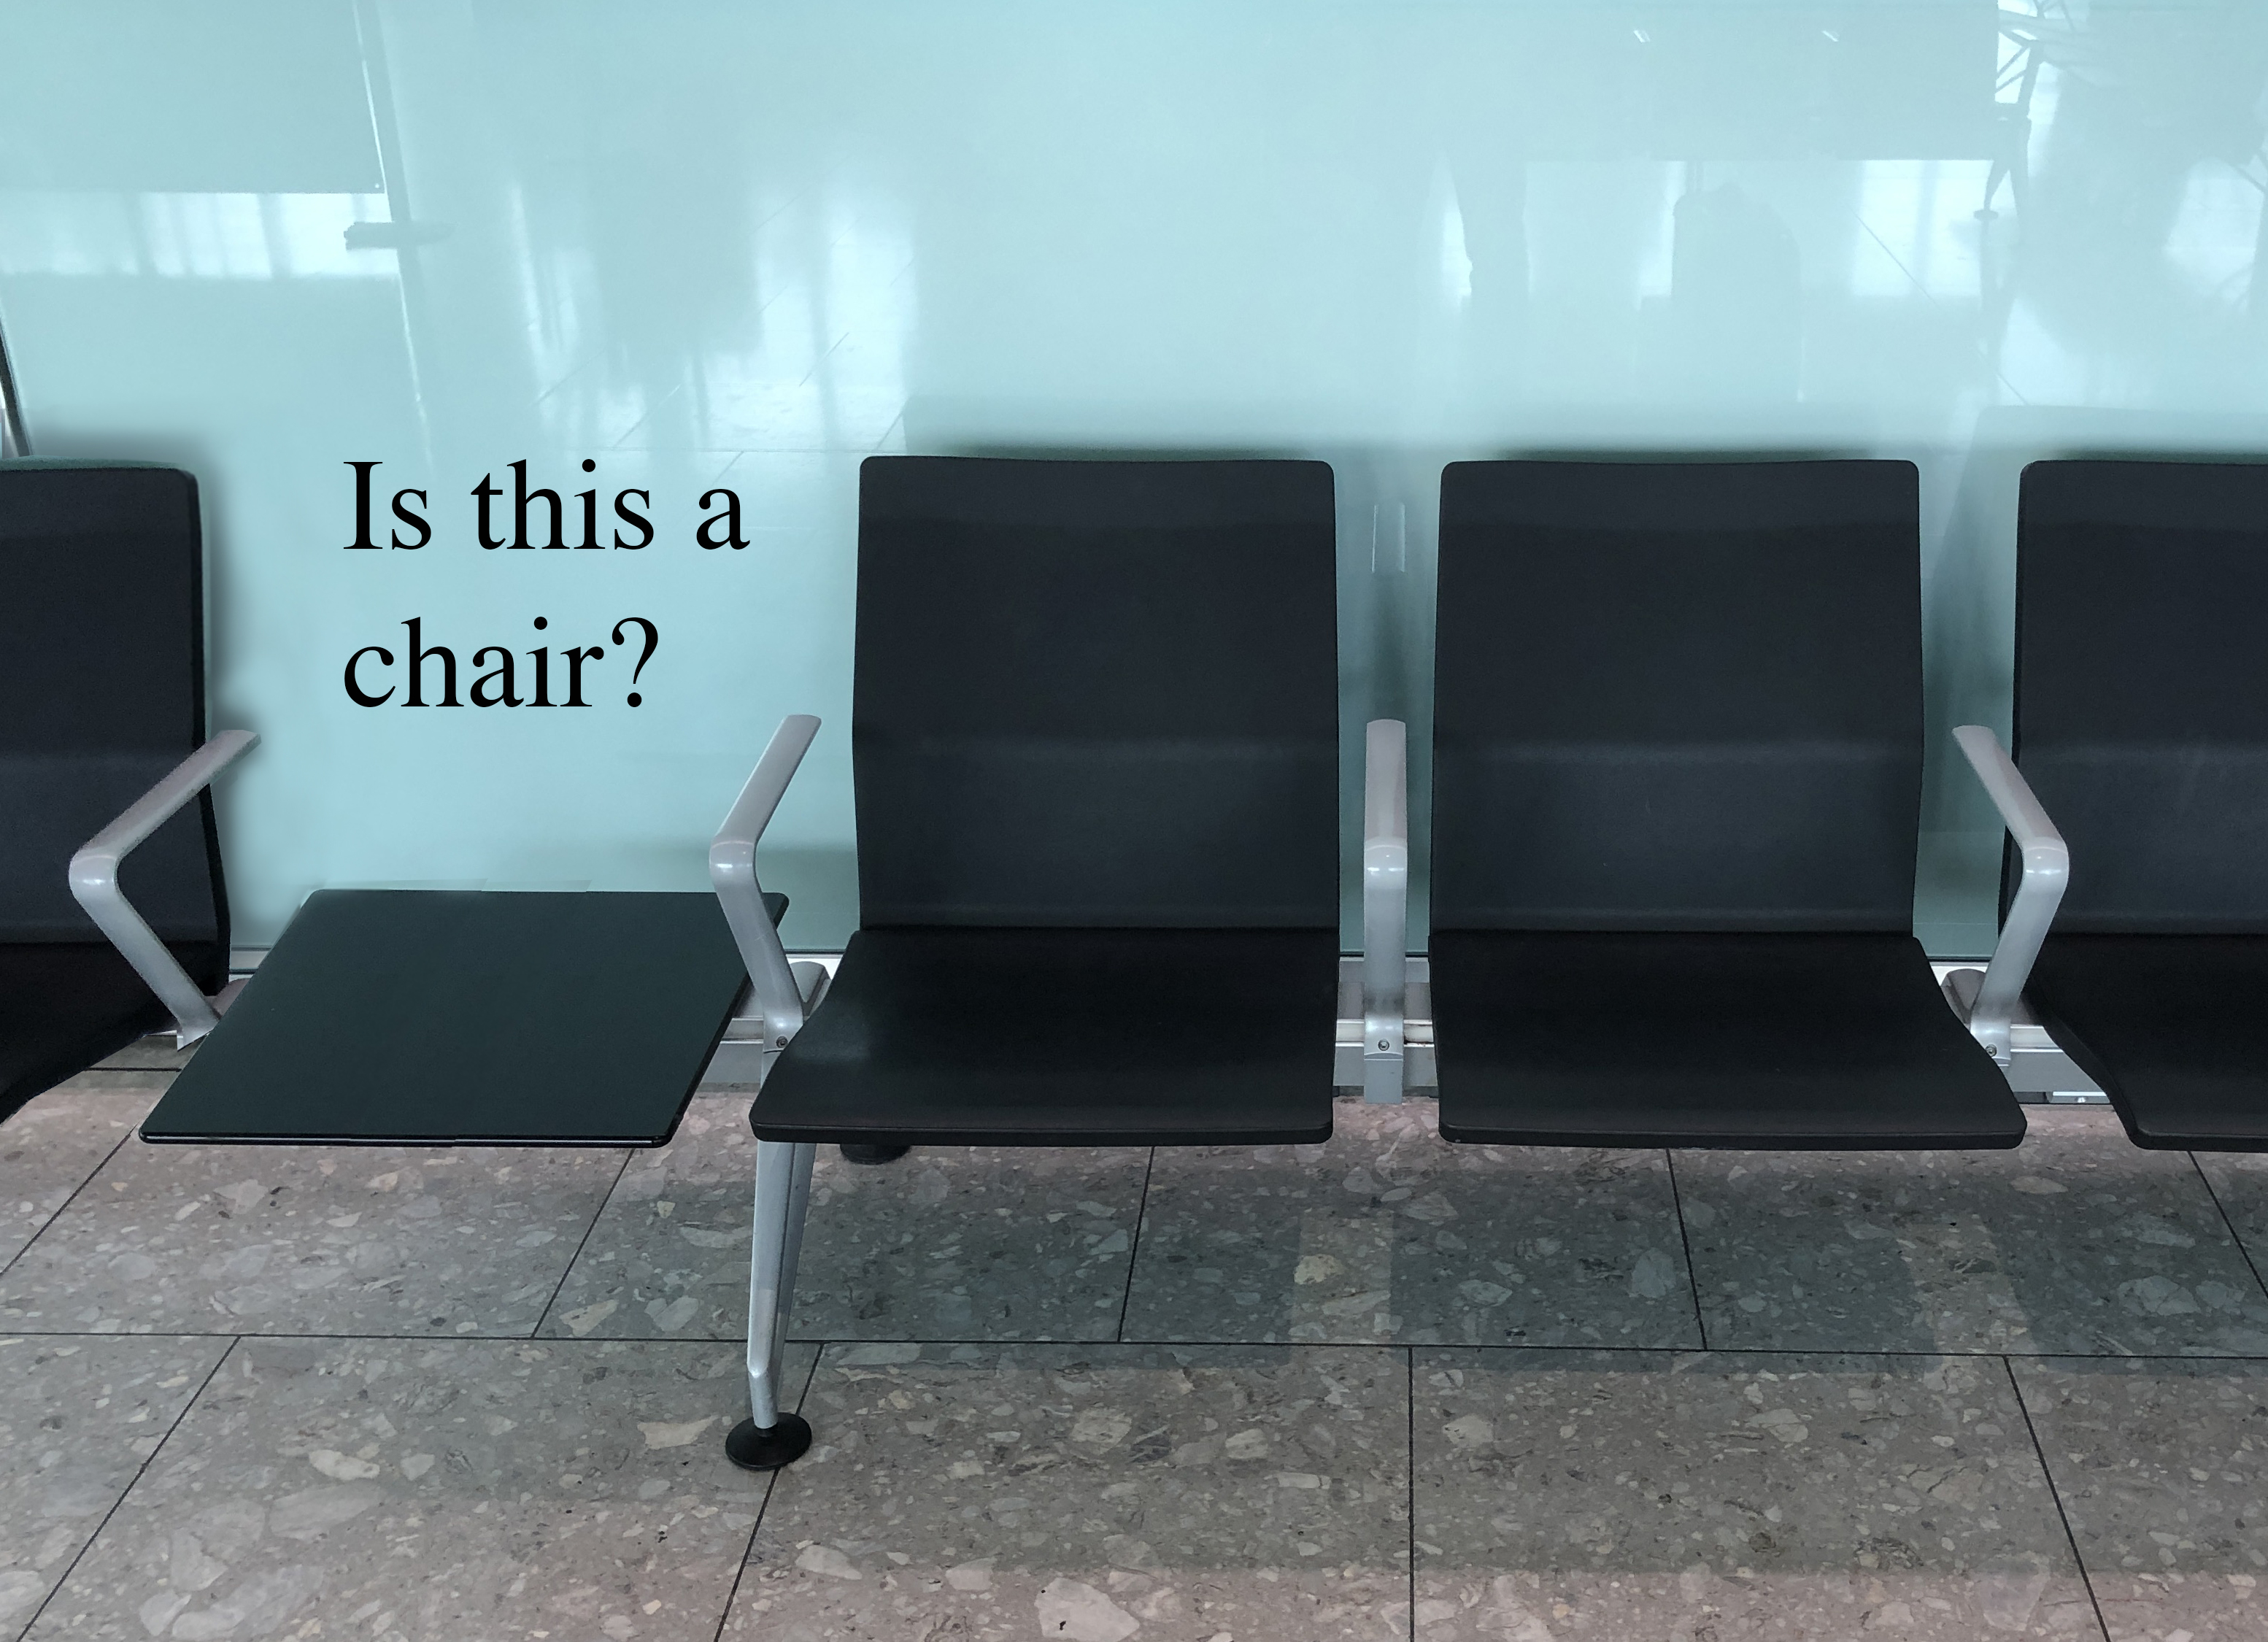
\includegraphics[width=0.7\linewidth]{figures/object_recognition/what_is_a_chair_with_text.jpg}
}
\caption{What is a chair? The definition is based on affordances (i.e., something you can sit on) and on social conventions (i.e., some surfaces you can sit on are meant to be used to support other objects than yourself). Affordances are likely to be directly accessible through vision, while social conventions might not be.}
\end{figure}

In this chapter we will study three tasks related to the recognition of objects in images (classification, localization, and segmentation). We will introduce the problem definitions and the formulation that lays the foundations for most existing approaches. 


% Different tasks require different outputs. 

%		FIGURE: show an image where the chair is clearly visible, and another with a chair in a busy  scene. 
%		Maybe  the rest could be: function and loss
%		image classification (is the object present somewhere?)
%		localization: bounding boxes
%		semantic segmentations: pixel labeling 
%		panoptic segmentation: segments and instances
%		instance identification (my chair vs a chair)
%		objects, parts, attributes, stuff

%Following blocks
%\begin{itemize}
%\item Task specification
%\item Representation
%\item Features
%\item Classifier
%\end{itemize}


%\begin{figure}[h]
%    \centering
%    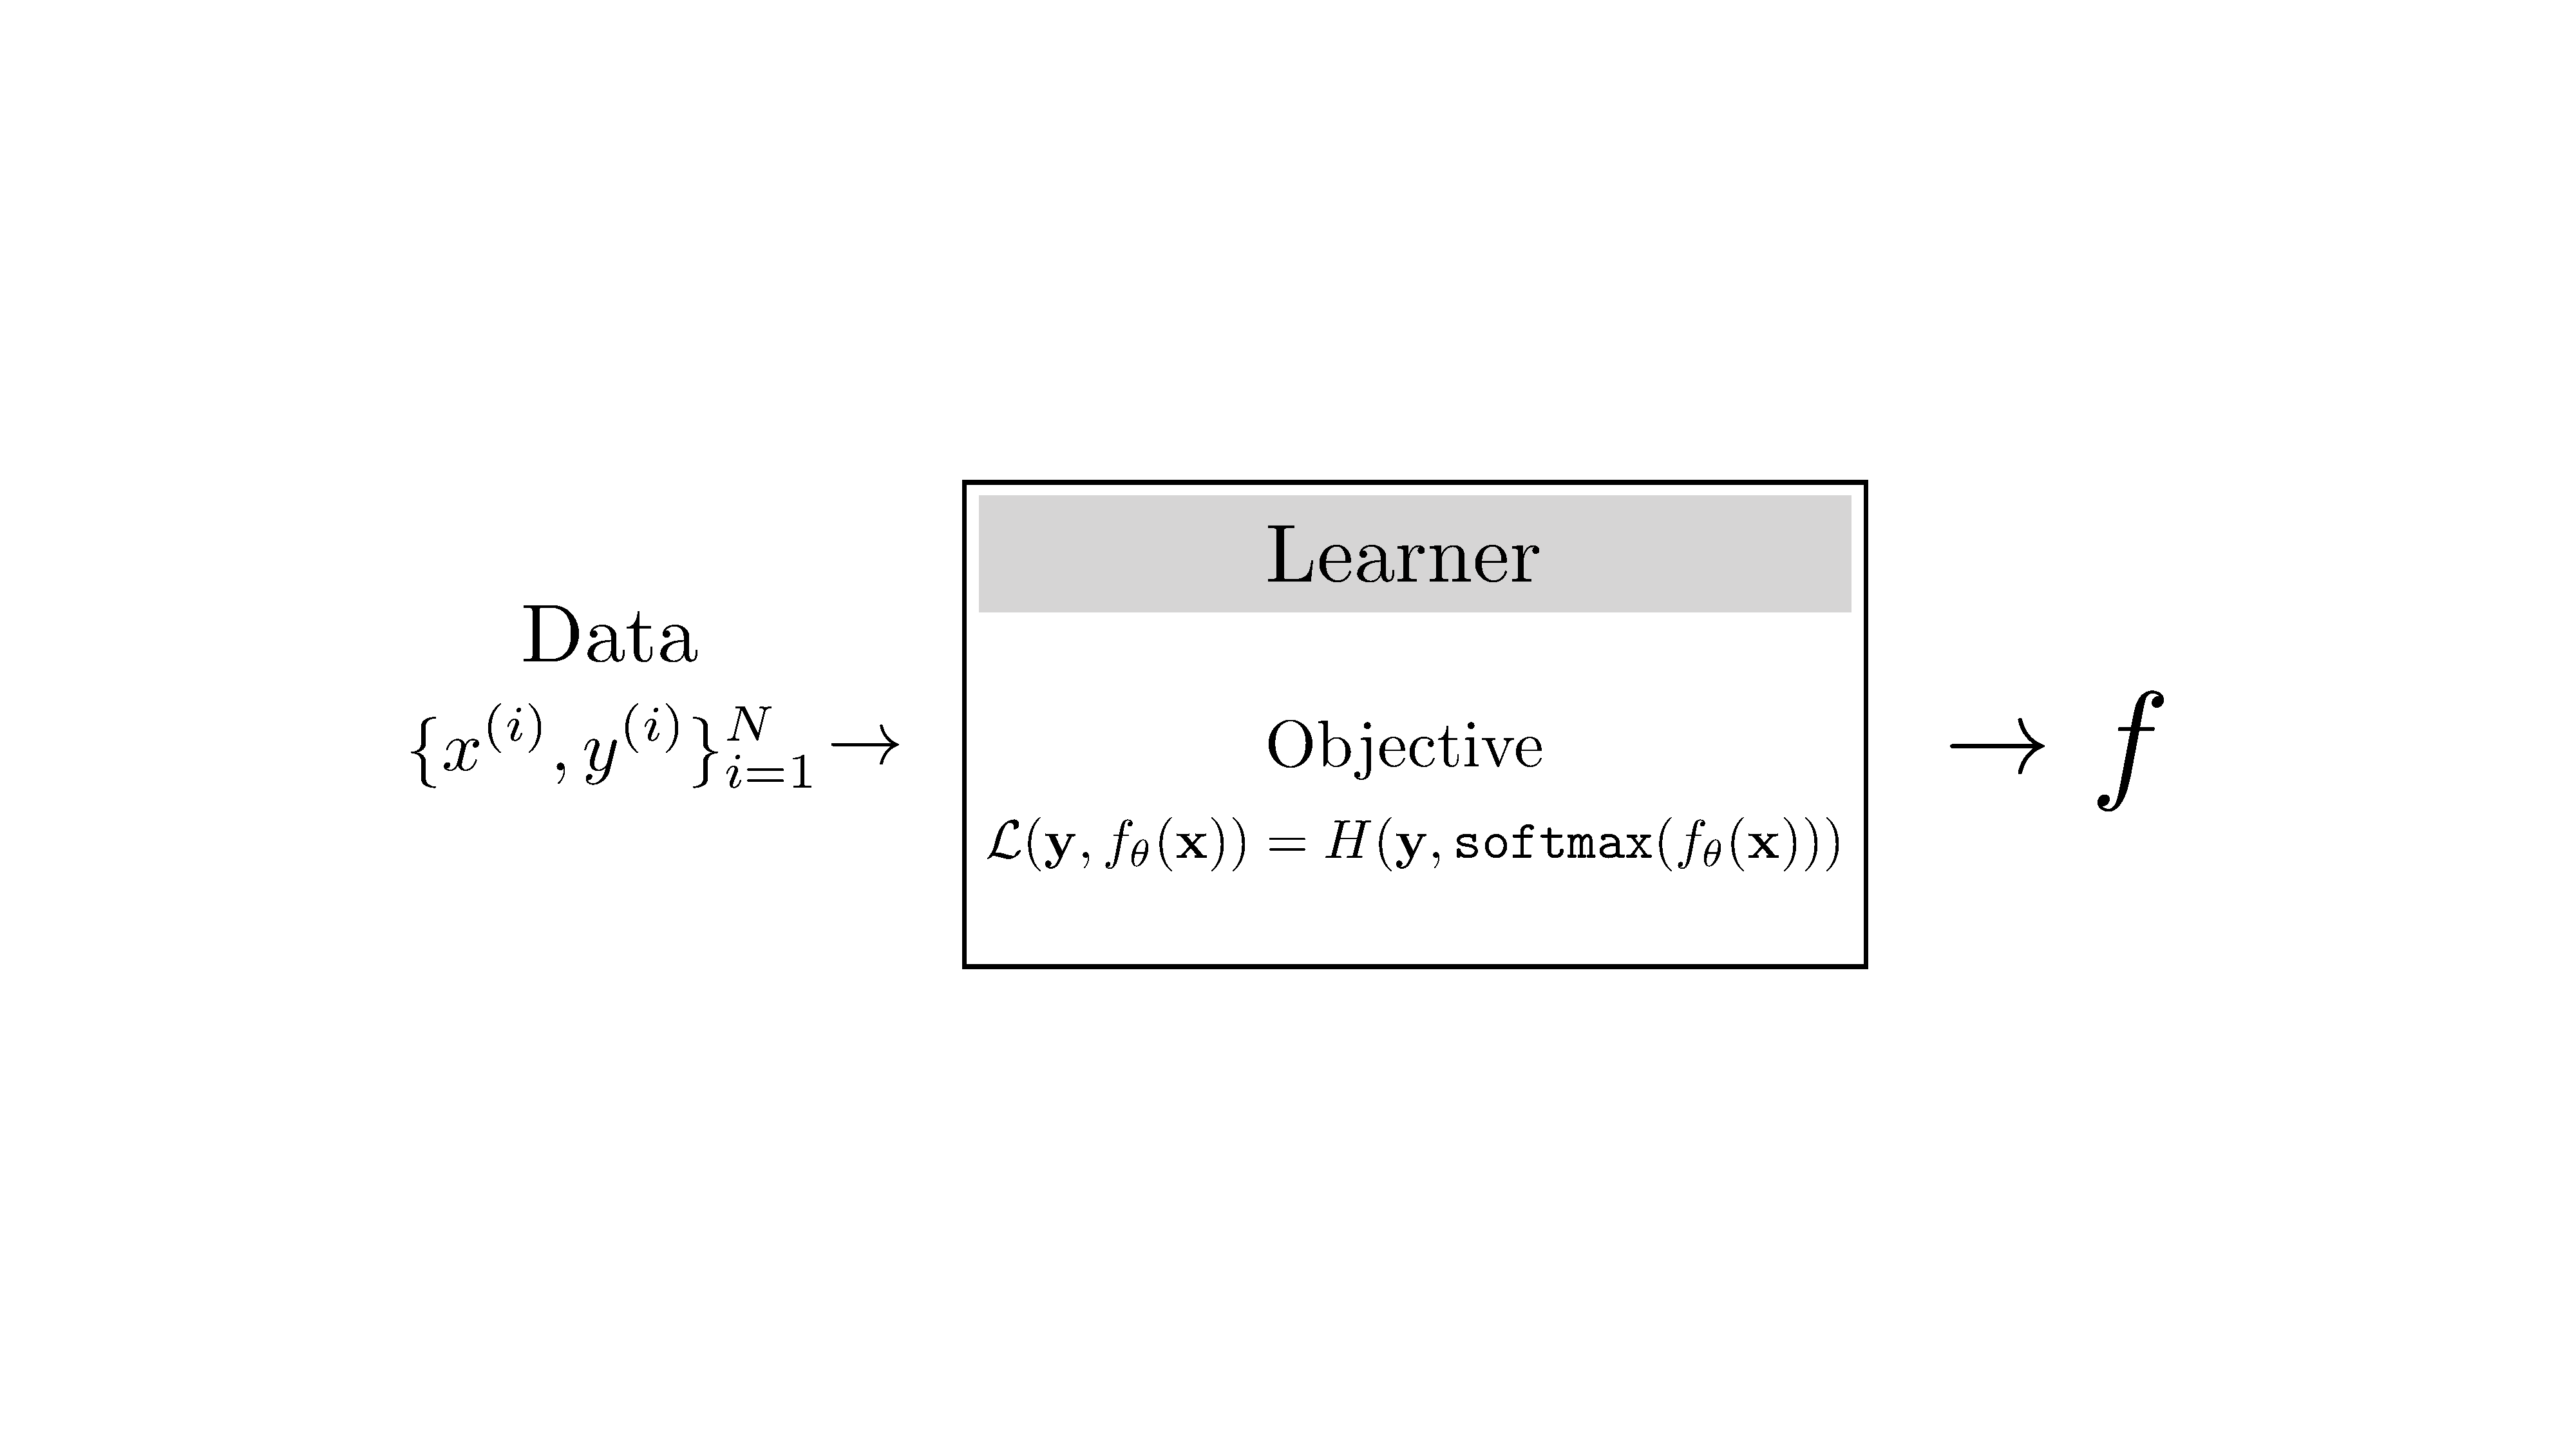
\includegraphics[width=0.7\linewidth]{./figures/intro_to_learning/softmax_regression_learning_problem.pdf}
%    \label{fig:softmax_regression_learning_problem}
%\end{figure}




\section{Image Classification}
\label{sec:image_classification}

%\subsection{Definition}

Image classification is one of the simplest tasks in object recognition. The goal is to answer the following, seemingly simple, question: Is object class $c$ present anywhere in the image ${\bf x}$?
\marginnote{We also covered image classification as a case study of machine learning in \sect{\ref{sec:intro_to_learning:image_classification}}. We repeat some of the technical material here, but go into more detail and focus on how image classification relates to different kinds of visual understanding.}[-0.4cm]

Image classification typically assumes that there is a closed vocabulary of object classes with a finite number of predefined classes. If our vocabulary contains $K$ classes, we can loop over the classes and ask the same question for each class. This task does not try to localize the object in the image, or to count how many instances of the object are present.
 
\subsection{Formulation}
%One canonical task in object recognition is to build a function $f$ that takes as input image $\bf x$? and answers the following question: {\bf is object class $c$ present anywhere in the image $\bf x$?} The output, $\hat {\bf y}$, of the function will be a binary response: $1=yes$ and $0=no$. 
We can answer the previous question in a mathematical form by building a function that maps the input image ${\bf x}$ into an output vector $\hat {\bf y}$:
\begin{equation}
\hat {\bf y} = f({\bf x})
\end{equation}
The output, $\hat {\bf y}$, of the function will be a binary response: $1=yes$, the object is present; and $0=no$, the object is not present. 

\begin{figure}
\centerline{
\includegraphics[width=0.5\linewidth]{figures/object_recognition/image_classification.eps}}
\caption{Image classification: Is there a car in this image?}
\end{figure}


In general we want to classify an image according to multiple classes. We can do this by having as output a vector $\hat {\bf y}$ of length $K$, where $K$ is the number of classes. Component $c$ of the vector $\hat {\bf y}$ will indicate whether class $c$ is present or absent in the image. For instance, the training set will be composed of examples of images and the corresponding class indicator vectors as shown in \fig{\ref{fig:classification_training_set}} (in this case, $K=3$).

\begin{figure}
\centerline{
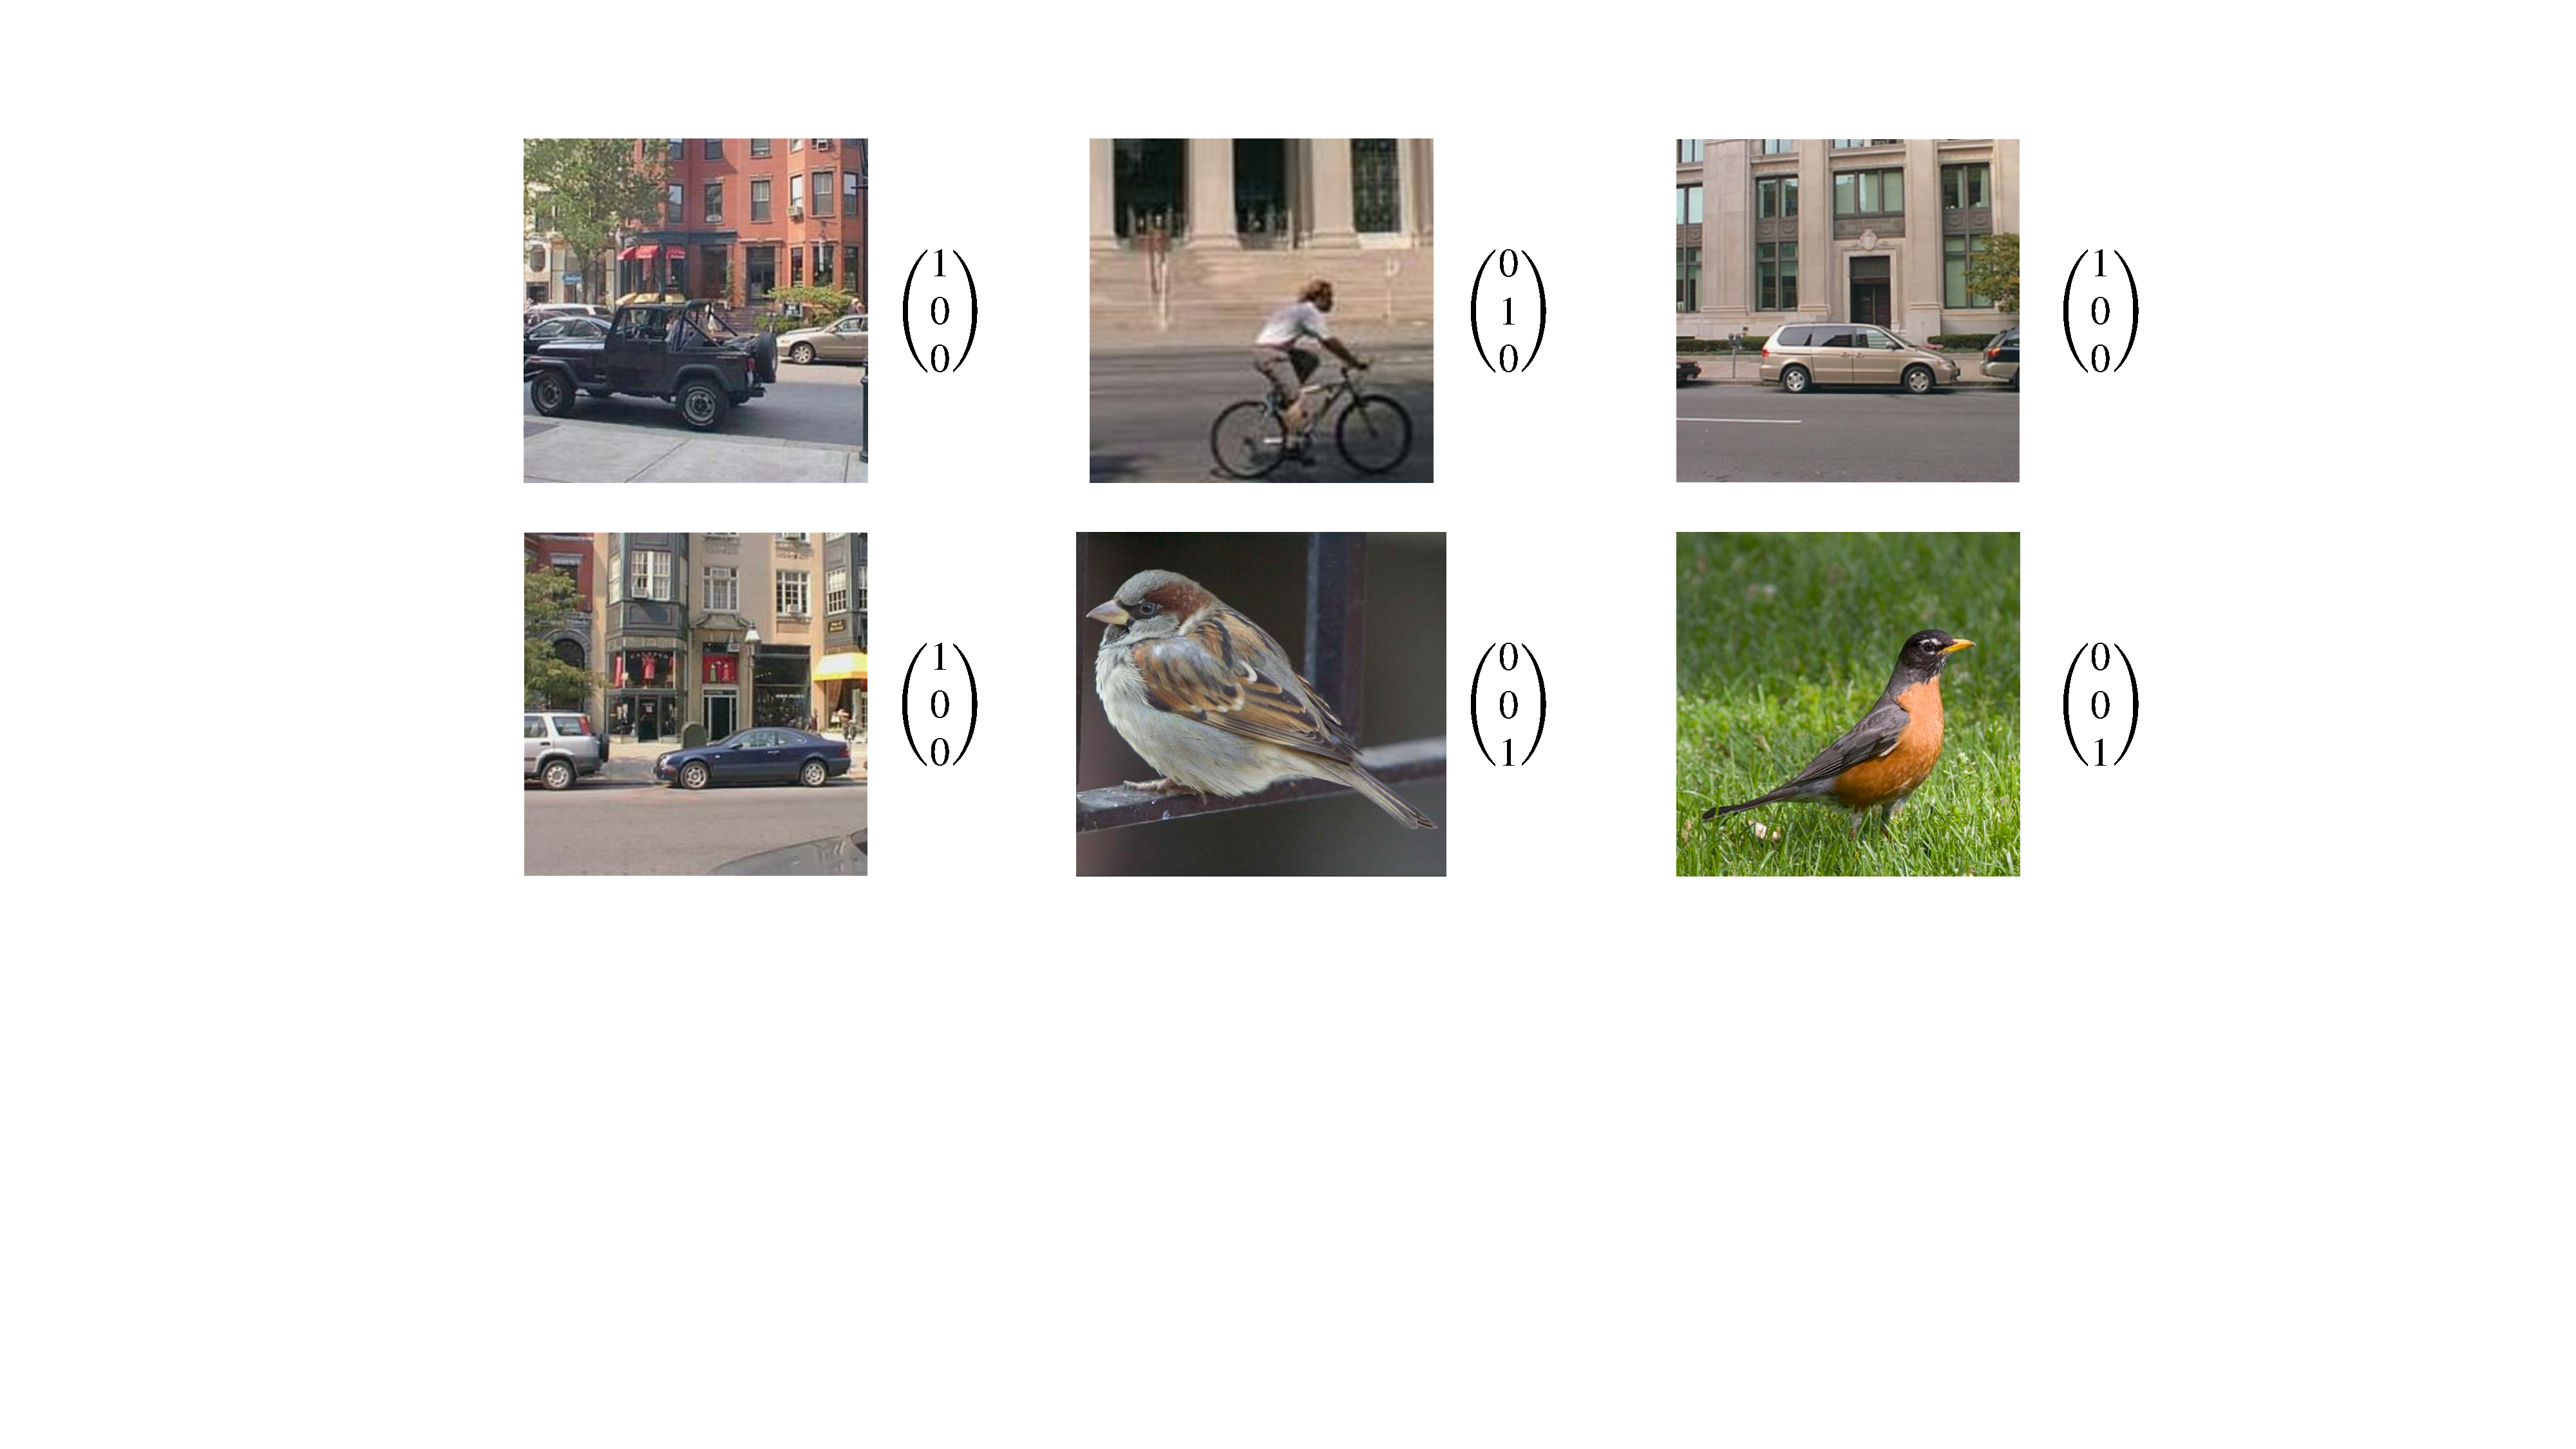
\includegraphics[width=1\linewidth]{figures/object_recognition/classification_training_set.pdf}
}
\caption{Training set for image classification with $K=3$ classes.}
\label{fig:classification_training_set}
\end{figure}

We want to enrich the output so that it also represents the uncertainty in the presence of the object. This uncertainty can be the result of a function $f$ that does not work very well, or from a noisy or blurry input image $\mathbf{x}$ where the object is difficult to see. One can formulate this as a function $f$ that takes as input the image ${\bf x}$ and outputs the probability distribution of the $K$ classes: $\hat{\mathbf{y}}=(y_1, y_2, ..., y_K)$, where $y_c$ is the probability that object class $c$ is present in the image $\mathbf{x}$:

\begin{equation}
\hat {\bf y}_c = p({\bf y}_c=1 \given {\bf x}, \theta) 
\end{equation}

\subsubsection{Exclusive classes}
%~\\

One common assumption is that only one class, among the $K$ possible classes, is present in the image. This is typical in settings where most of the images contain a single large object.   
Multiclass classification with exclusive classes results is given in the following constraint: 
\begin{equation}
\sum_{c=1}^K \hat{y}_c=1
\end{equation}
where $0>\hat{y}_c>1$.
In the toy example with three classes shown previously, the valid solutions for $\mathbf{y}=(y_1, y_2, y_3)$ are constrained to lie within a \textbf{simplex}.\marginnote{Simplex with three exclusive classes.
\\~\\
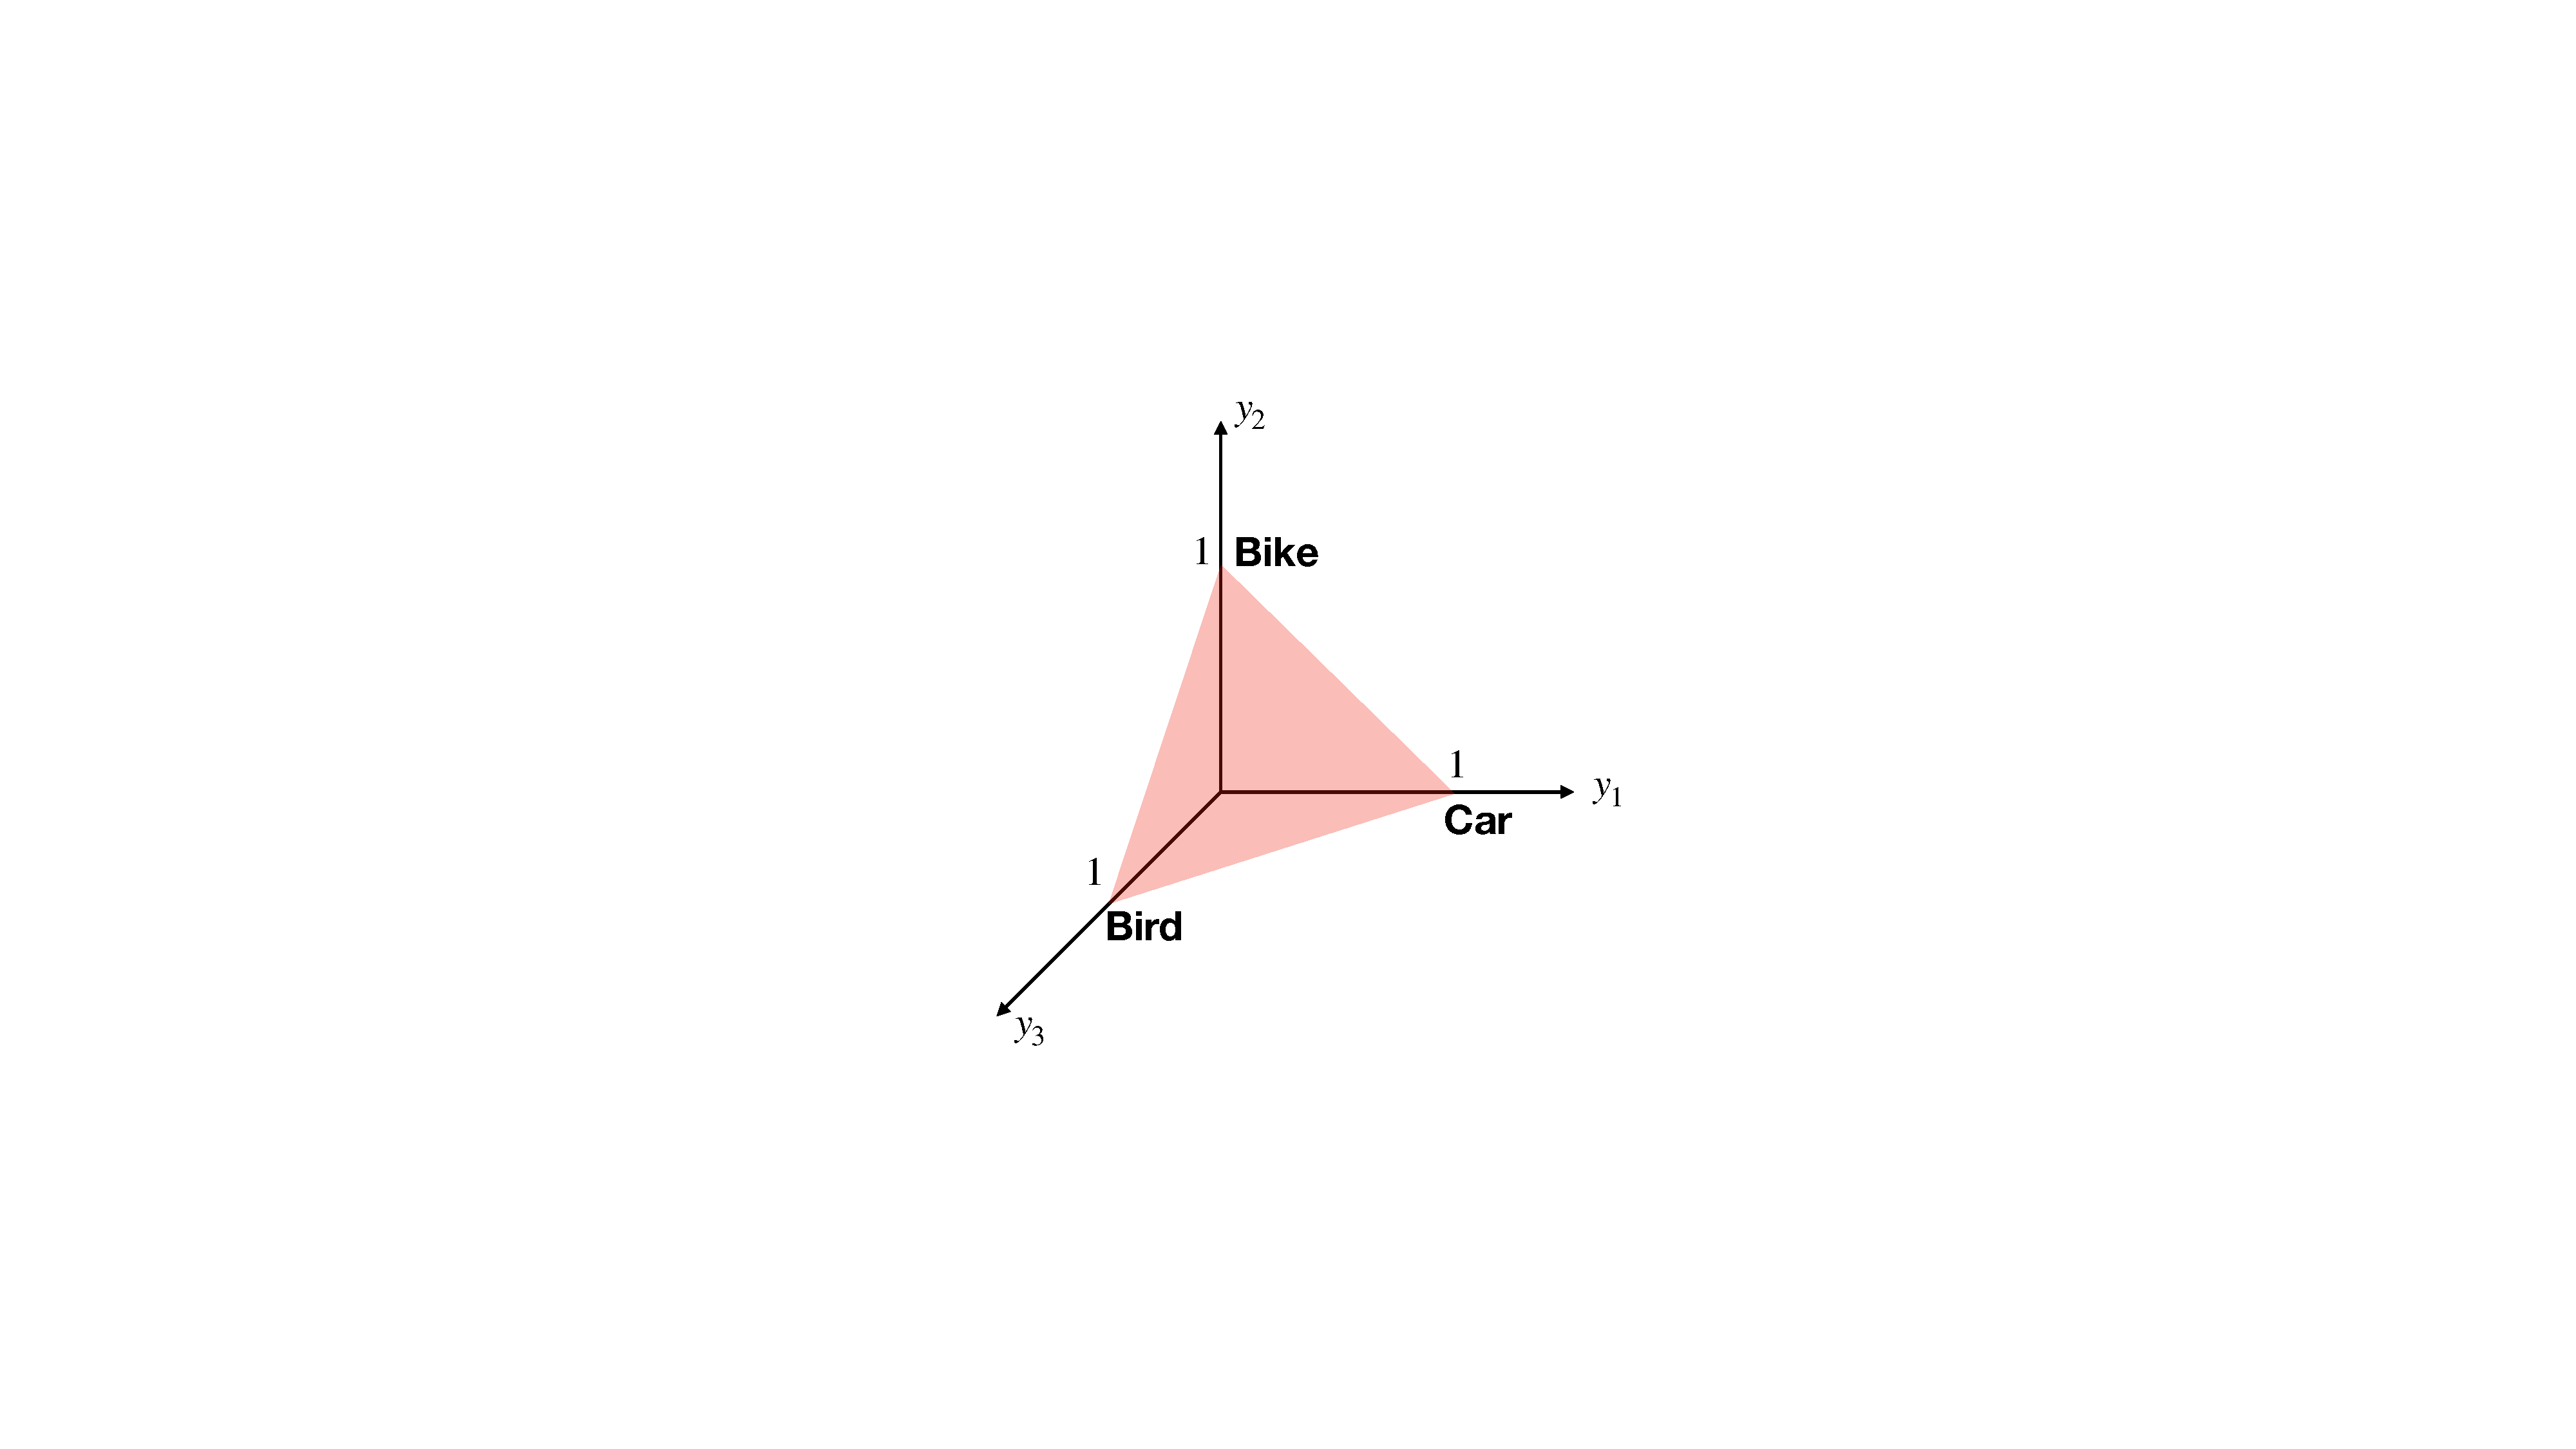
\includegraphics[width=1\linewidth]{figures/object_recognition/simplex.pdf}
}
Under this formulation, the function $f$ is a mapping $f:\mathbb{R}^{N \times M \times 3} \rightarrow \mathbb{S}^K$ from the set of red-green-blue (RGB) images to the $K$-dimensional simplex, $\mathbb{S}^K$. 

%\subsection{Architecture}

The function $f$ is constrained to belong to a family of possible functions. For instance, $f$ might belong to the space of all the functions that can be built with a neural network. In such a case the function is specified by the network parameters $\theta: f_\theta$. When using a neural net, the vector $\hat{\mathbf{y}}$ is usually computed as the output of a softmax layer. 

\subsubsection{Multilabel classification}
%~\\

When the image can have multiple labels simultaneously, the classification problem can be formulated as $K$ binary classification problems (where $K$ is the number of classes). 

In such a case, the function $f_\theta$ can be a neural network shared across all classes (\fig{\ref{fig:class_architecture}}), and the output vector $\hat{\mathbf{y}}$, of length $K$, is computed using a sigmoid nonlinearity for each output class. In this case the output can still be interpreted as the probability $\hat {\bf y}_c = p({\bf y}_c=1 \given {\bf x}, \theta)$, but without the constraint that the sum across classes to be 1. 


\begin{figure}
\centerline{
\includegraphics[width=0.7\linewidth]{figures/object_recognition/class_architecture.eps}}
\caption{Multilabel image classification system.}
\label{fig:class_architecture}
\end{figure}

\subsection{Classification Loss}

In order to learn the model parameters, we need to define the loss function that will capture the task that we want to solve. One natural measure of classification error is the {\bf missclassication error}. The errors that the function $f$ makes are the number of misplaced 1's (i.e., the  misclassification error) over the dataset, which we can write as:

\begin{align}
    \mathcal{L}(\hat{\mathbf{y}},\mathbf{y}) =
    \sum_{t=1}^T \sum_{c=1}^{K}
    \mathbbm{1}(\hat{y}^{(t)}_c \neq y^{(t)}_c ).
\end{align}

However, it is hard to learn the function parameters using gradient descent with this loss as it is not differentiable. Finding the optimal parameters of function $f_\theta$ requires defining a loss function that we will be tractable to optimize during the training stage. 
%Loss function: 
%The probability of the ground truth data under the output distribution: 

\subsubsection{Exclusive classes}
%~\\

If we interpret the function $f$ as estimating the probability $p({\bf y}_c=1 \given {\bf x}, \theta) = \hat {\bf y}_c$, with $\sum_c \hat {\bf y}_c =1$. The likelihood of the ground truth data is:
\begin{equation}
\prod_{t=1}^T \prod_{c=1}^K \left( \hat {\bf y}^{(t)}_c \right) ^{{\bf y}^{(t)}_c}\label{eqn:object_recognition:classification_likelihood}
\end{equation}

%\begin{align}
%    \mathcal{L}(\hat{\mathbf{y}},\mathbf{y}) = H(\mathbf{y}, \hat{\mathbf{y}}) = - \sum_{k=1}^K y_k \log \hat{y}_k.
%\end{align}

where the first product loops over all $T$ training examples, and the second product loops over all the classes $K$. We want to find the parameters $\theta$ that maximize the likelihood of the ground truth labels for whole training image. As we have seen in \chap{\ref{chapter:convolutional_neural_nets}}, maximizing the likelihood corresponds to minimizing the {\bf cross entropy loss} (which we get by just taking the negative log of the  equation [\ref{eqn:object_recognition:classification_likelihood}]), resulting in a total classification loss:
\begin{equation}
    \mathcal{L}_{cls}(\hat{\mathbf{y}},\mathbf{y})
     = -\sum_{t=1}^{T} \sum_{c=1}^{K} y^{(t)}_c \log(\hat{y}^{(t)}_c)
\end{equation}

The cross-entropy loss is differentiable and it is commonly used in image classification tasks. 

\subsubsection{Multilabel classification}
%~\\

If classes are not exclusive, the likelihood of the ground truth data is:
\begin{equation}
\prod_{t=1}^T \prod_{c=1}^K \left( \hat {\bf y}^{(t)}_c \right) ^{{\bf y}^{(t)}_c}
\left( 1-\hat {\bf y}^{(t)}_c \right) ^{1-{\bf y}^{(t)}_c}
\end{equation}
\marginnote{Bernoulli distribution: The binary random variable $y$ takes the value 1 with probability $a$ and the value 0 with probability $1-a$. The probability $y$ can be written as $p(y) = a^y (1-a)^{1-y}$.}
where the outputs $\hat {\bf y}_c$ are computed using a sigmoid layer.  Taking the negative log of the likelihood gives the {\bf multiclass binary cross-entropy loss}:

\begin{equation}
    \mathcal{L}_{cls}(\hat{\mathbf{y}},\mathbf{y})
     = -\sum_{t=1}^{T} \sum_{c=1}^{K} y^{(t)}_c \log(\hat{y}^{(t)}_c)
     + 
     (1-y^{(t)}_c) \log(1-\hat{y}^{(t)}_c)
\end{equation}



%\marginnote{Cross entropy loss: pictorial description of how it works.}

%\subsection{Architecture}

%The function $f$ is constrained to belong to a family of possible functions. For instance, $f$ might belong to the space of all the functions that can be built with a neural network. In such a case the function is specified by the network parameters $\theta: f_\theta$. When using a neural net, the vector $\hat{\mathbf{y}}$ is usually computed as the output of a softmax layer. 

\subsection{Evaluation}

Once the function $f_\theta$ has been trained, we have to evaluate its performance over a holdout test set. There are several popular measures of performance:

Classification performance uses the output of the classifier, $f$, as a continuous value, the score $\hat{y}_c$, for each class. We can rank the predicted classes according to that value. The {\bf top-1} performance measures the percentage of times that the true class-label matches the highest scored prediction, $\hat{y} = \underset{c}{\mathrm{argmax}} ( \hat{y}_c )$, in the test set: 

\begin{equation}
    \text{TOP-1} = \frac{100}{T}
    \sum_{t=1}^T \mathbbm{1}( \hat{y}^{(t)} = y^{(t)}) 
\end{equation}

In some benchmarks (such as ImageNet), researchers also measure the {\bf top-5} performance, which is the percentage of times that the true label is within the set of five highest scoring predictions. Top-5 is useful in settings where the labels might be ambiguous, or where multiple labels for one image might be possible. In the case of multiple labels, ideally, the test set should specify which labels are possible and evaluate only using those. The top-5 measure is less precise and it is used when the test set only contains one label despite that multiple labels might be correct. 

For multiclass prediction problems it is often useful to look at what is the structure of mistakes made by the model. The {\bf confusion matrix} summarizes both the overall performance of the classifier and also the percentage of times that two classes are confused by the classifier. For instance, the following matrix shows the evaluation of a three-way classifier. The diagonal elements are the same as the top-1 performance for each class. The off-diagonal elements show the confusions. In this case, it seems that the classifier confuses cats as dogs the most. 
\begin{table}[h]
\marginnote{{\bf Table \ref{table:confusion_matrix}}: Confusion matrix for a three-way classification task. The numbers are percentages. } 
\faketablecaption{} 
\label{table:confusion_matrix}
%\begin{tabular}{|l|r|r|r|r|r|r|}
\begin{center}
\begin{tabular}{l|l|c|c|c|c}
\multicolumn{2}{c}{}&\multicolumn{3}{c}{Predicted class}&\\
\cline{3-5}
\multicolumn{2}{c|}{}&Cat&Car&Dog&\multicolumn{1}{c}{}\\
\cline{2-5}
& Cat & $80$ & $5$ & $15$ & $\rightarrow \sum = 100$\\
\cline{2-5}
True class & Car & $2$ & $95$ & $3$ & $\rightarrow \sum = 100$\\
\cline{2-5}
& Dog & $4$ & $0$ & $96$ & $\rightarrow \sum = 100$\\
\cline{2-5}
\end{tabular}
\end{center}
\end{table}
The elements of the confusion matrix are:
\begin{equation}
    C_{i,j} = 100 \frac{
    \sum_{t=1}^T \mathbbm{1}( \hat{y}^{(t)} = j)  \mathbbm{1} (y^{(t)} = i)
    }{
    \sum_{t=1}^T \mathbbm{1}(y^{(t)} = i) 
    }
\end{equation}
where $C_{i,j}$ measures the percentage of times that true class $i$ is classified as class $j$. 

In this toy example (\tab{\ref{table:confusion_matrix}}), we can see that 80 percent of the cat images are correctly classified, while 5 percent of cat images are classified as car images, and 15 percent are classified as pictures of dogs.
%classification performance
%Confusion matrix
%Precision-recall


% \subsection{Localization}

% Despite that the classifier has only been trained to detect the presence or absence of an object, it is possible that it has also learned to localize it in the image despite that it has not been explicitly trained to do so. 

% Backpropagate, CAM


\subsection{Shortcomings}

The task of image classification is plagued with issues. Although it is a useful task to measure progress in computer vision and machine learning, one has to be aware of its limitations when trying to use it to produce a meaningful description of a scene, or when developing a classifier for consumption in the real world.  

One very important shortcoming of this task is that it assumes that we can actually answer unambiguously the question {\em does the image contains object c?} But what happens if class definitions are ambiguous or class boundaries are soft? Even in cases were we believe that the boundaries might be well defined, it is east to find images that will challenge our assumption, as shown in \fig{\ref{fig:whatisacar}}.

\begin{figure}[t]
\centerline{
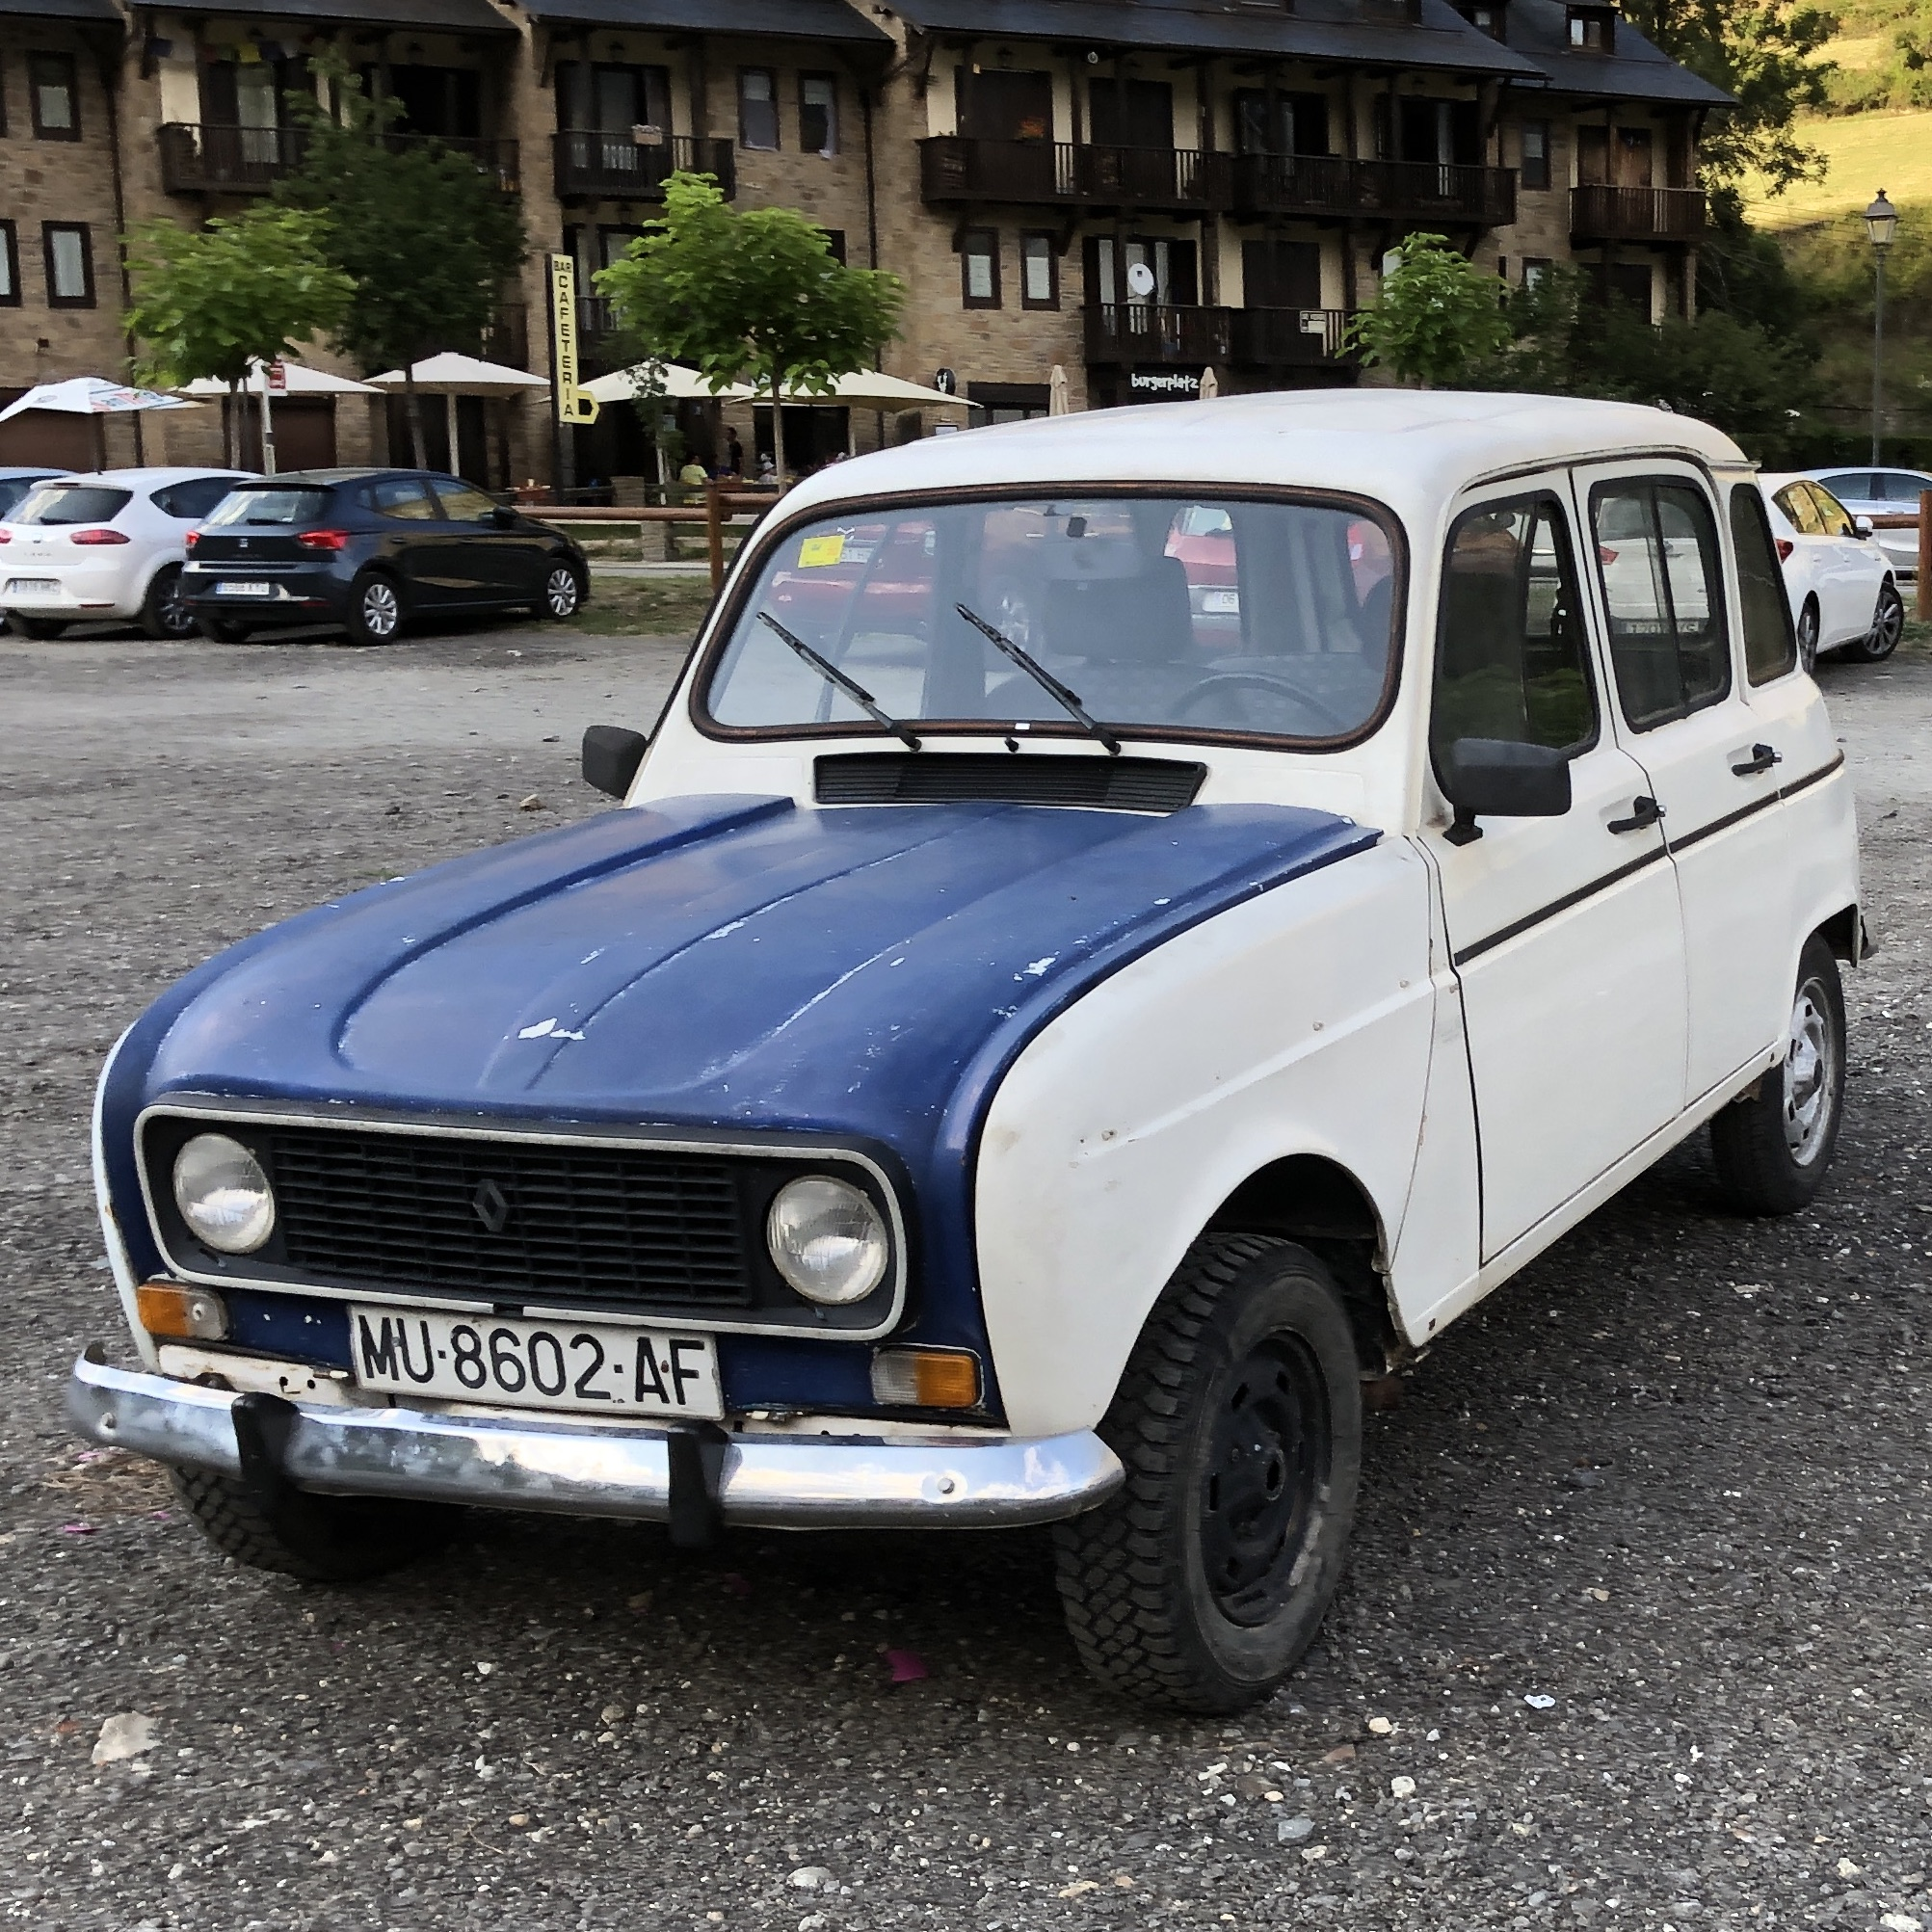
\includegraphics[width=0.32\linewidth]{figures/object_recognition/IMG_1260.jpeg}
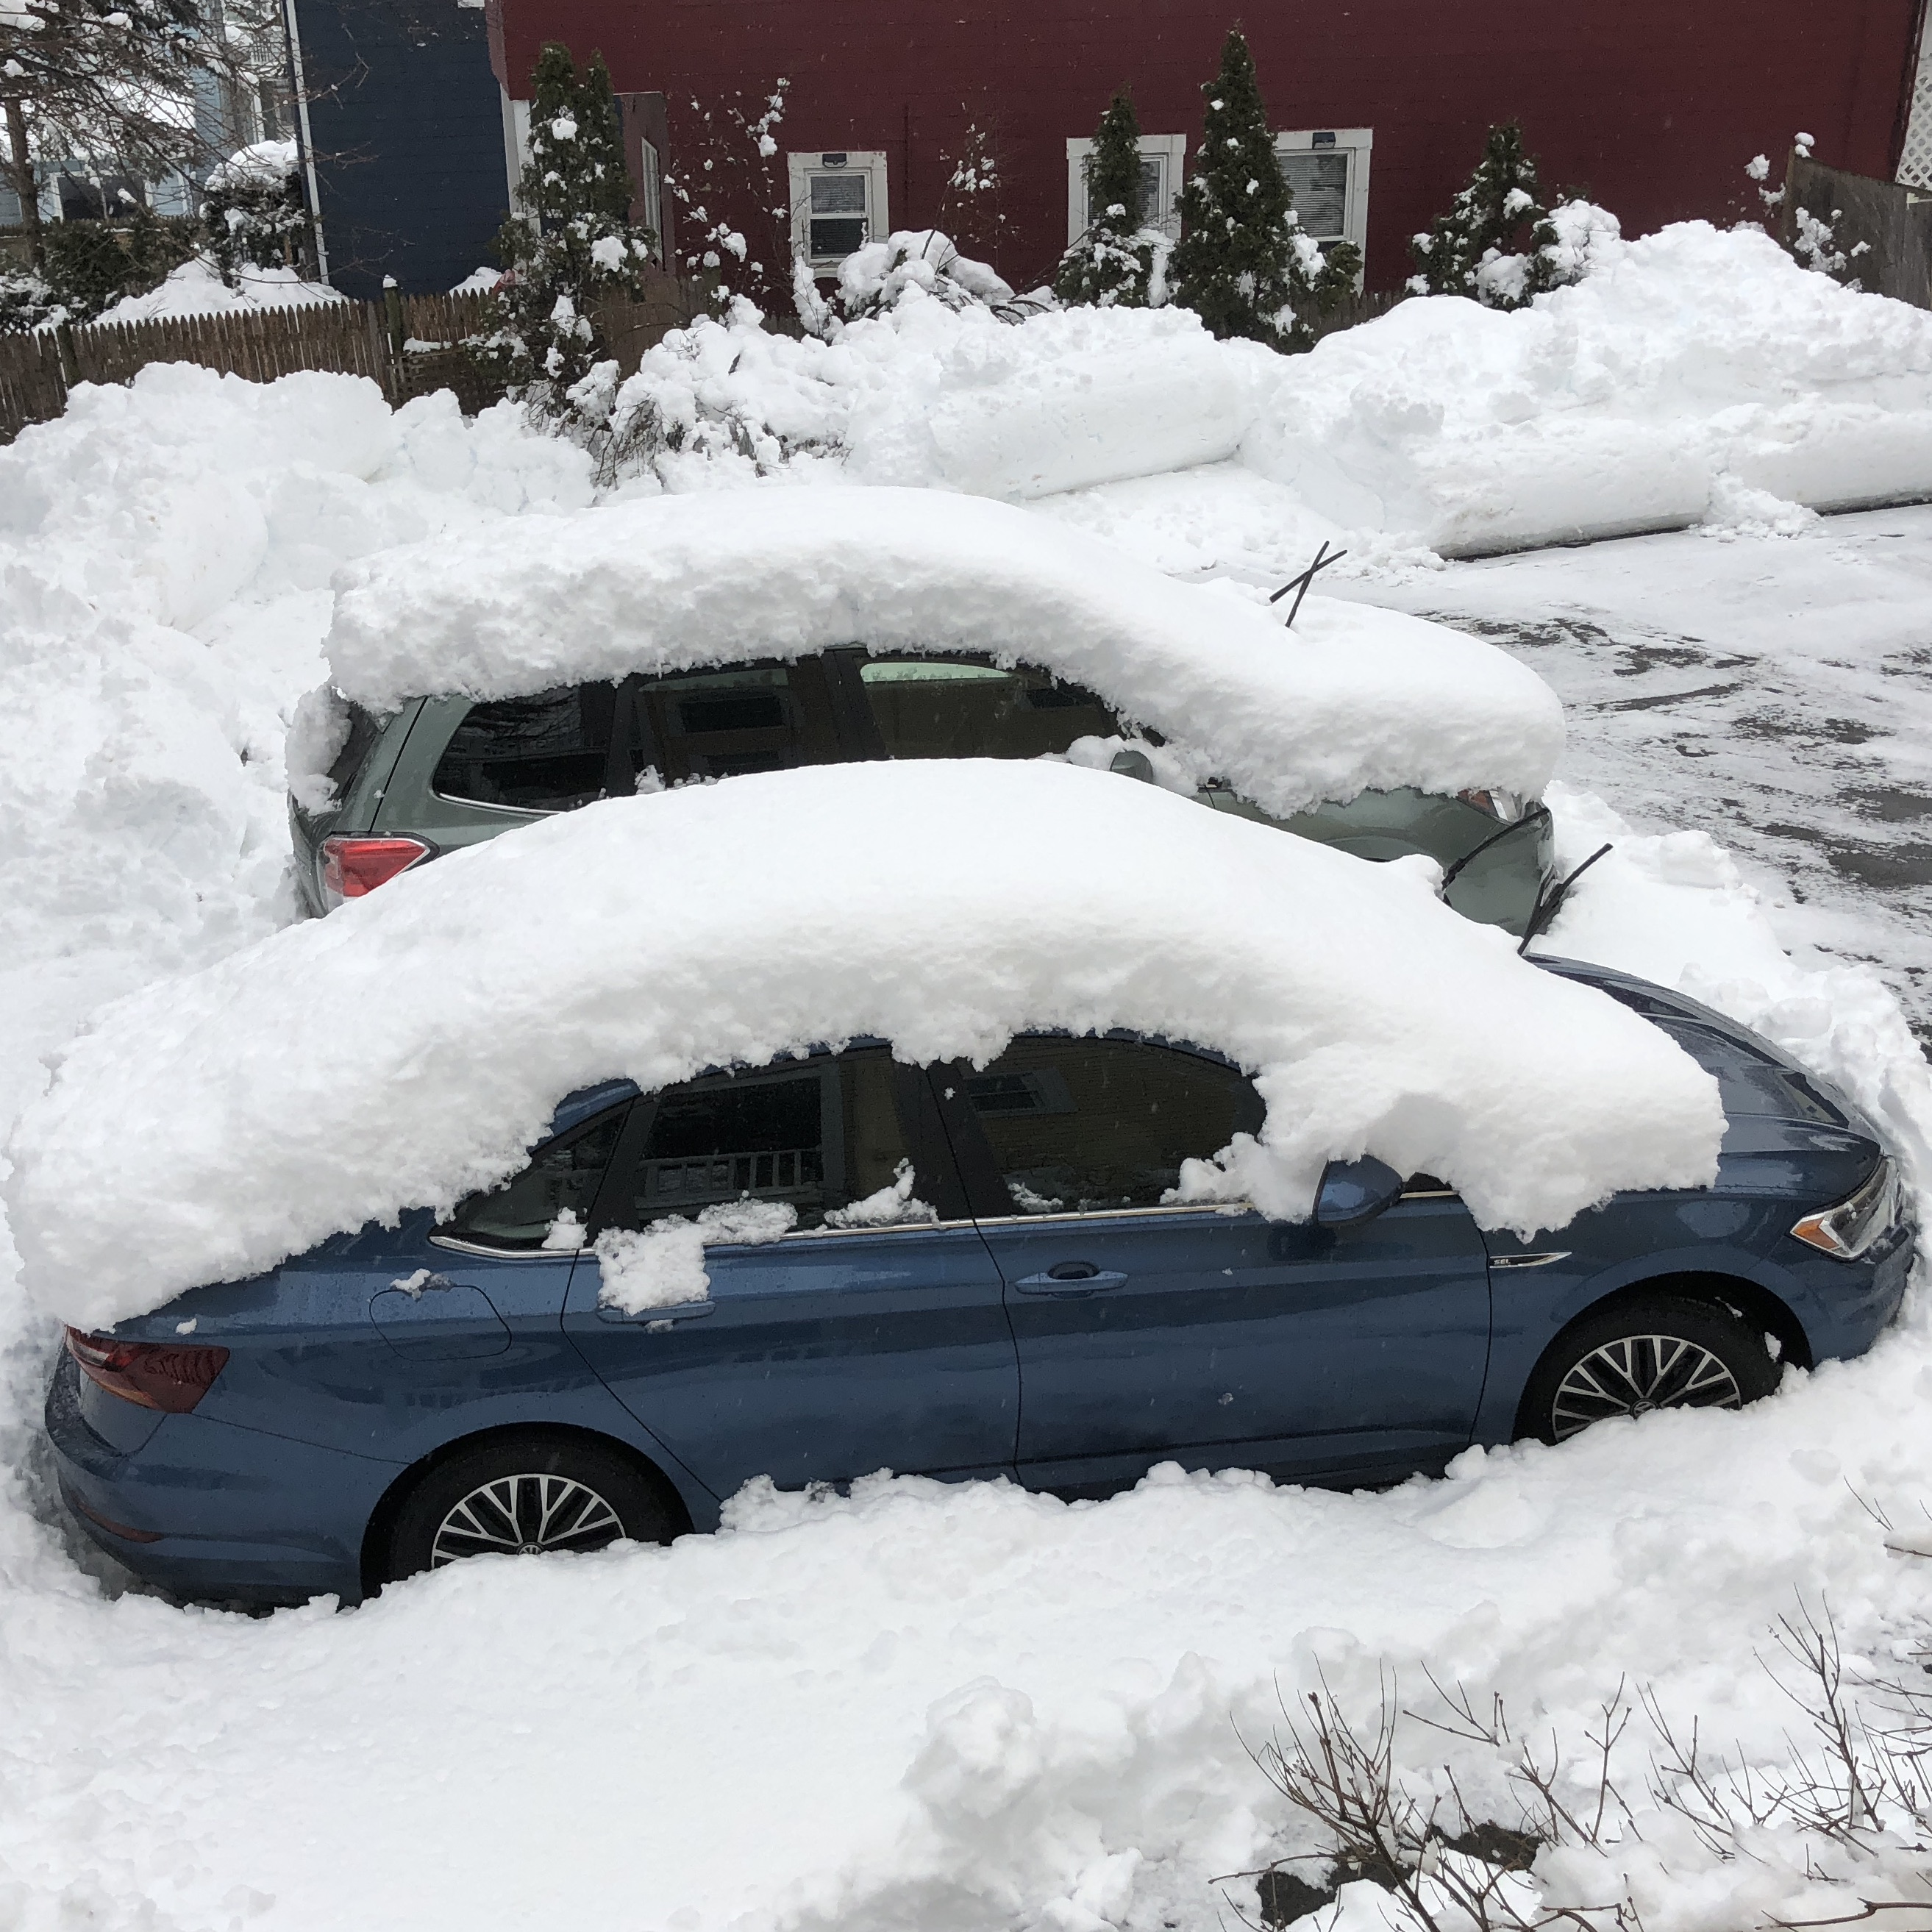
\includegraphics[width=0.32\linewidth]{figures/object_recognition/IMG_7095.jpeg}
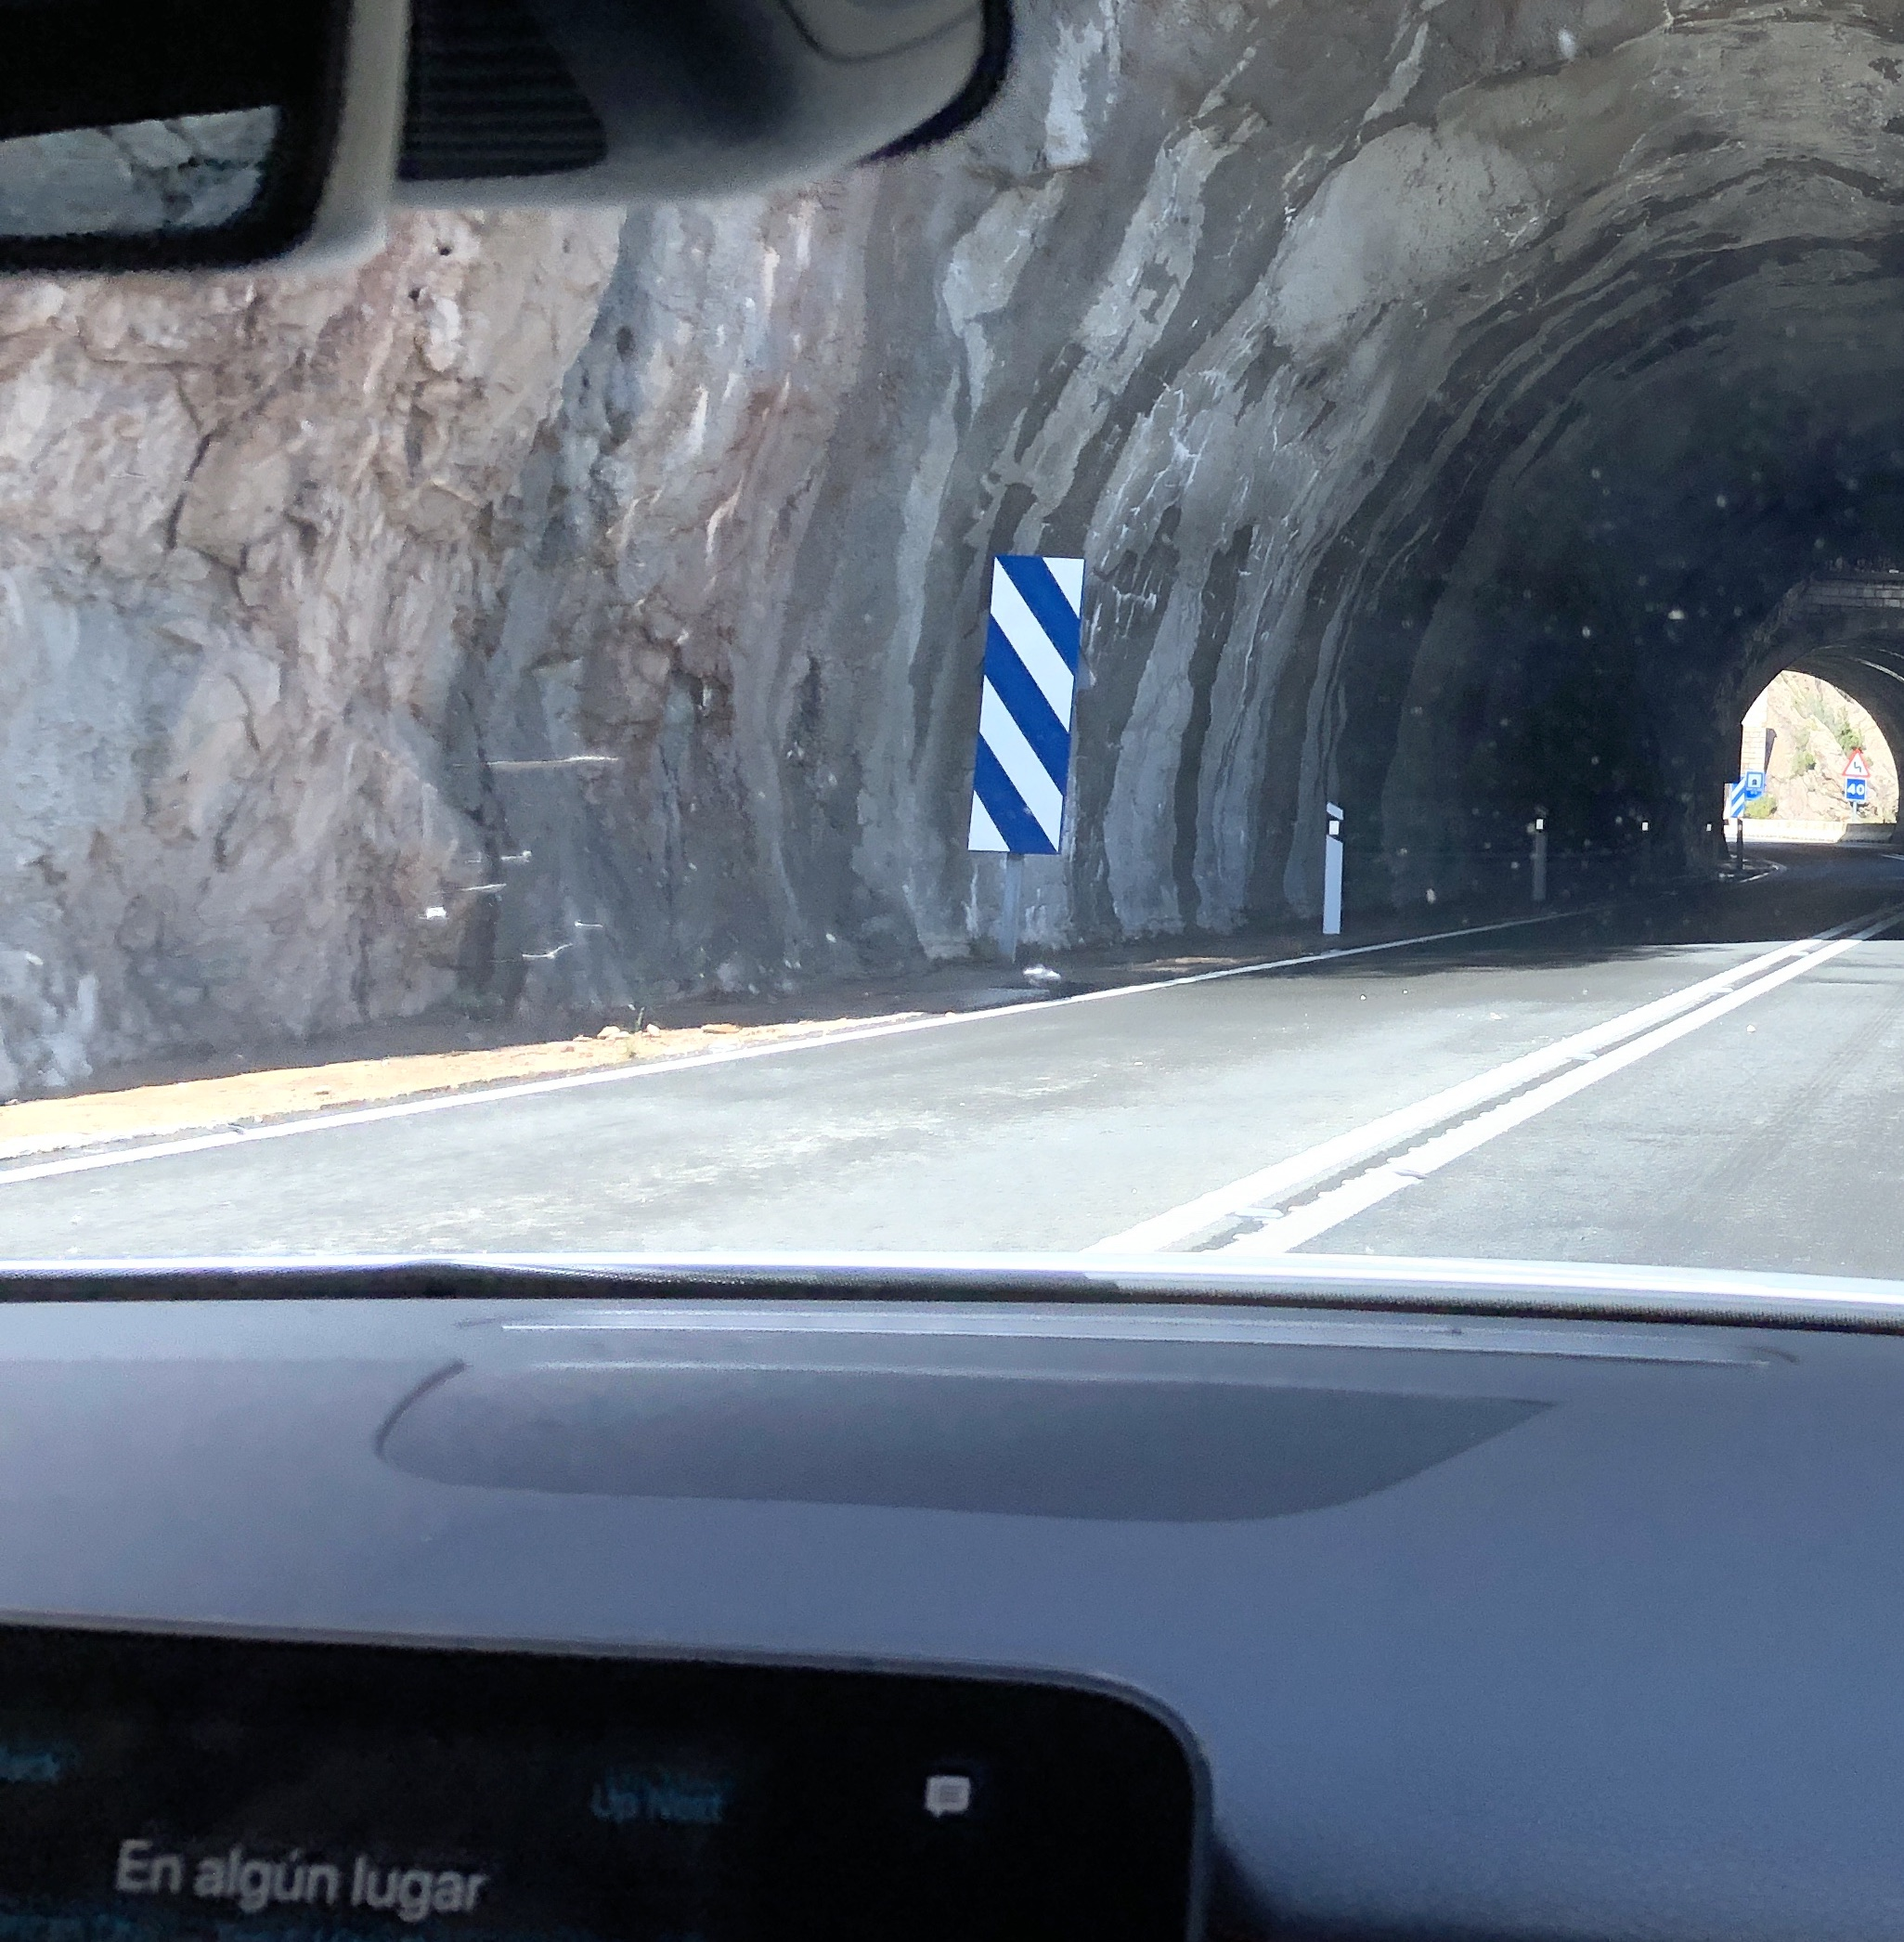
\includegraphics[width=0.32\linewidth]{figures/object_recognition/IMG_9933.jpeg}
}
\centerline{
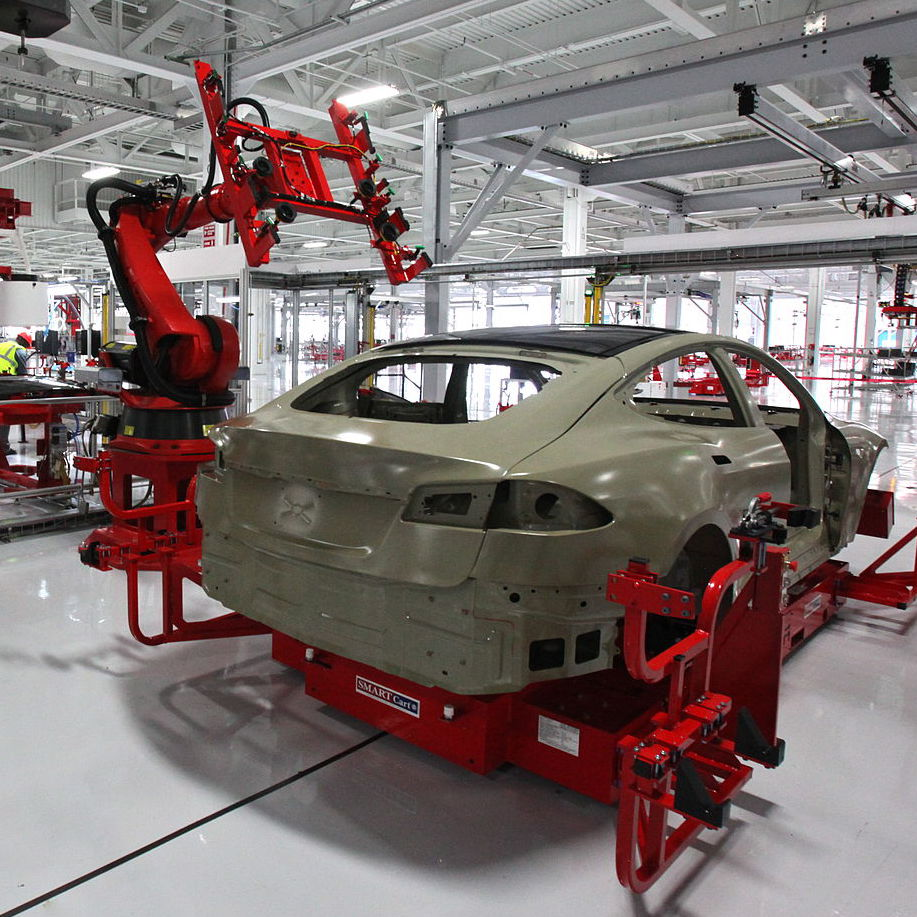
\includegraphics[width=0.32\linewidth]{figures/object_recognition/tesla.jpg}
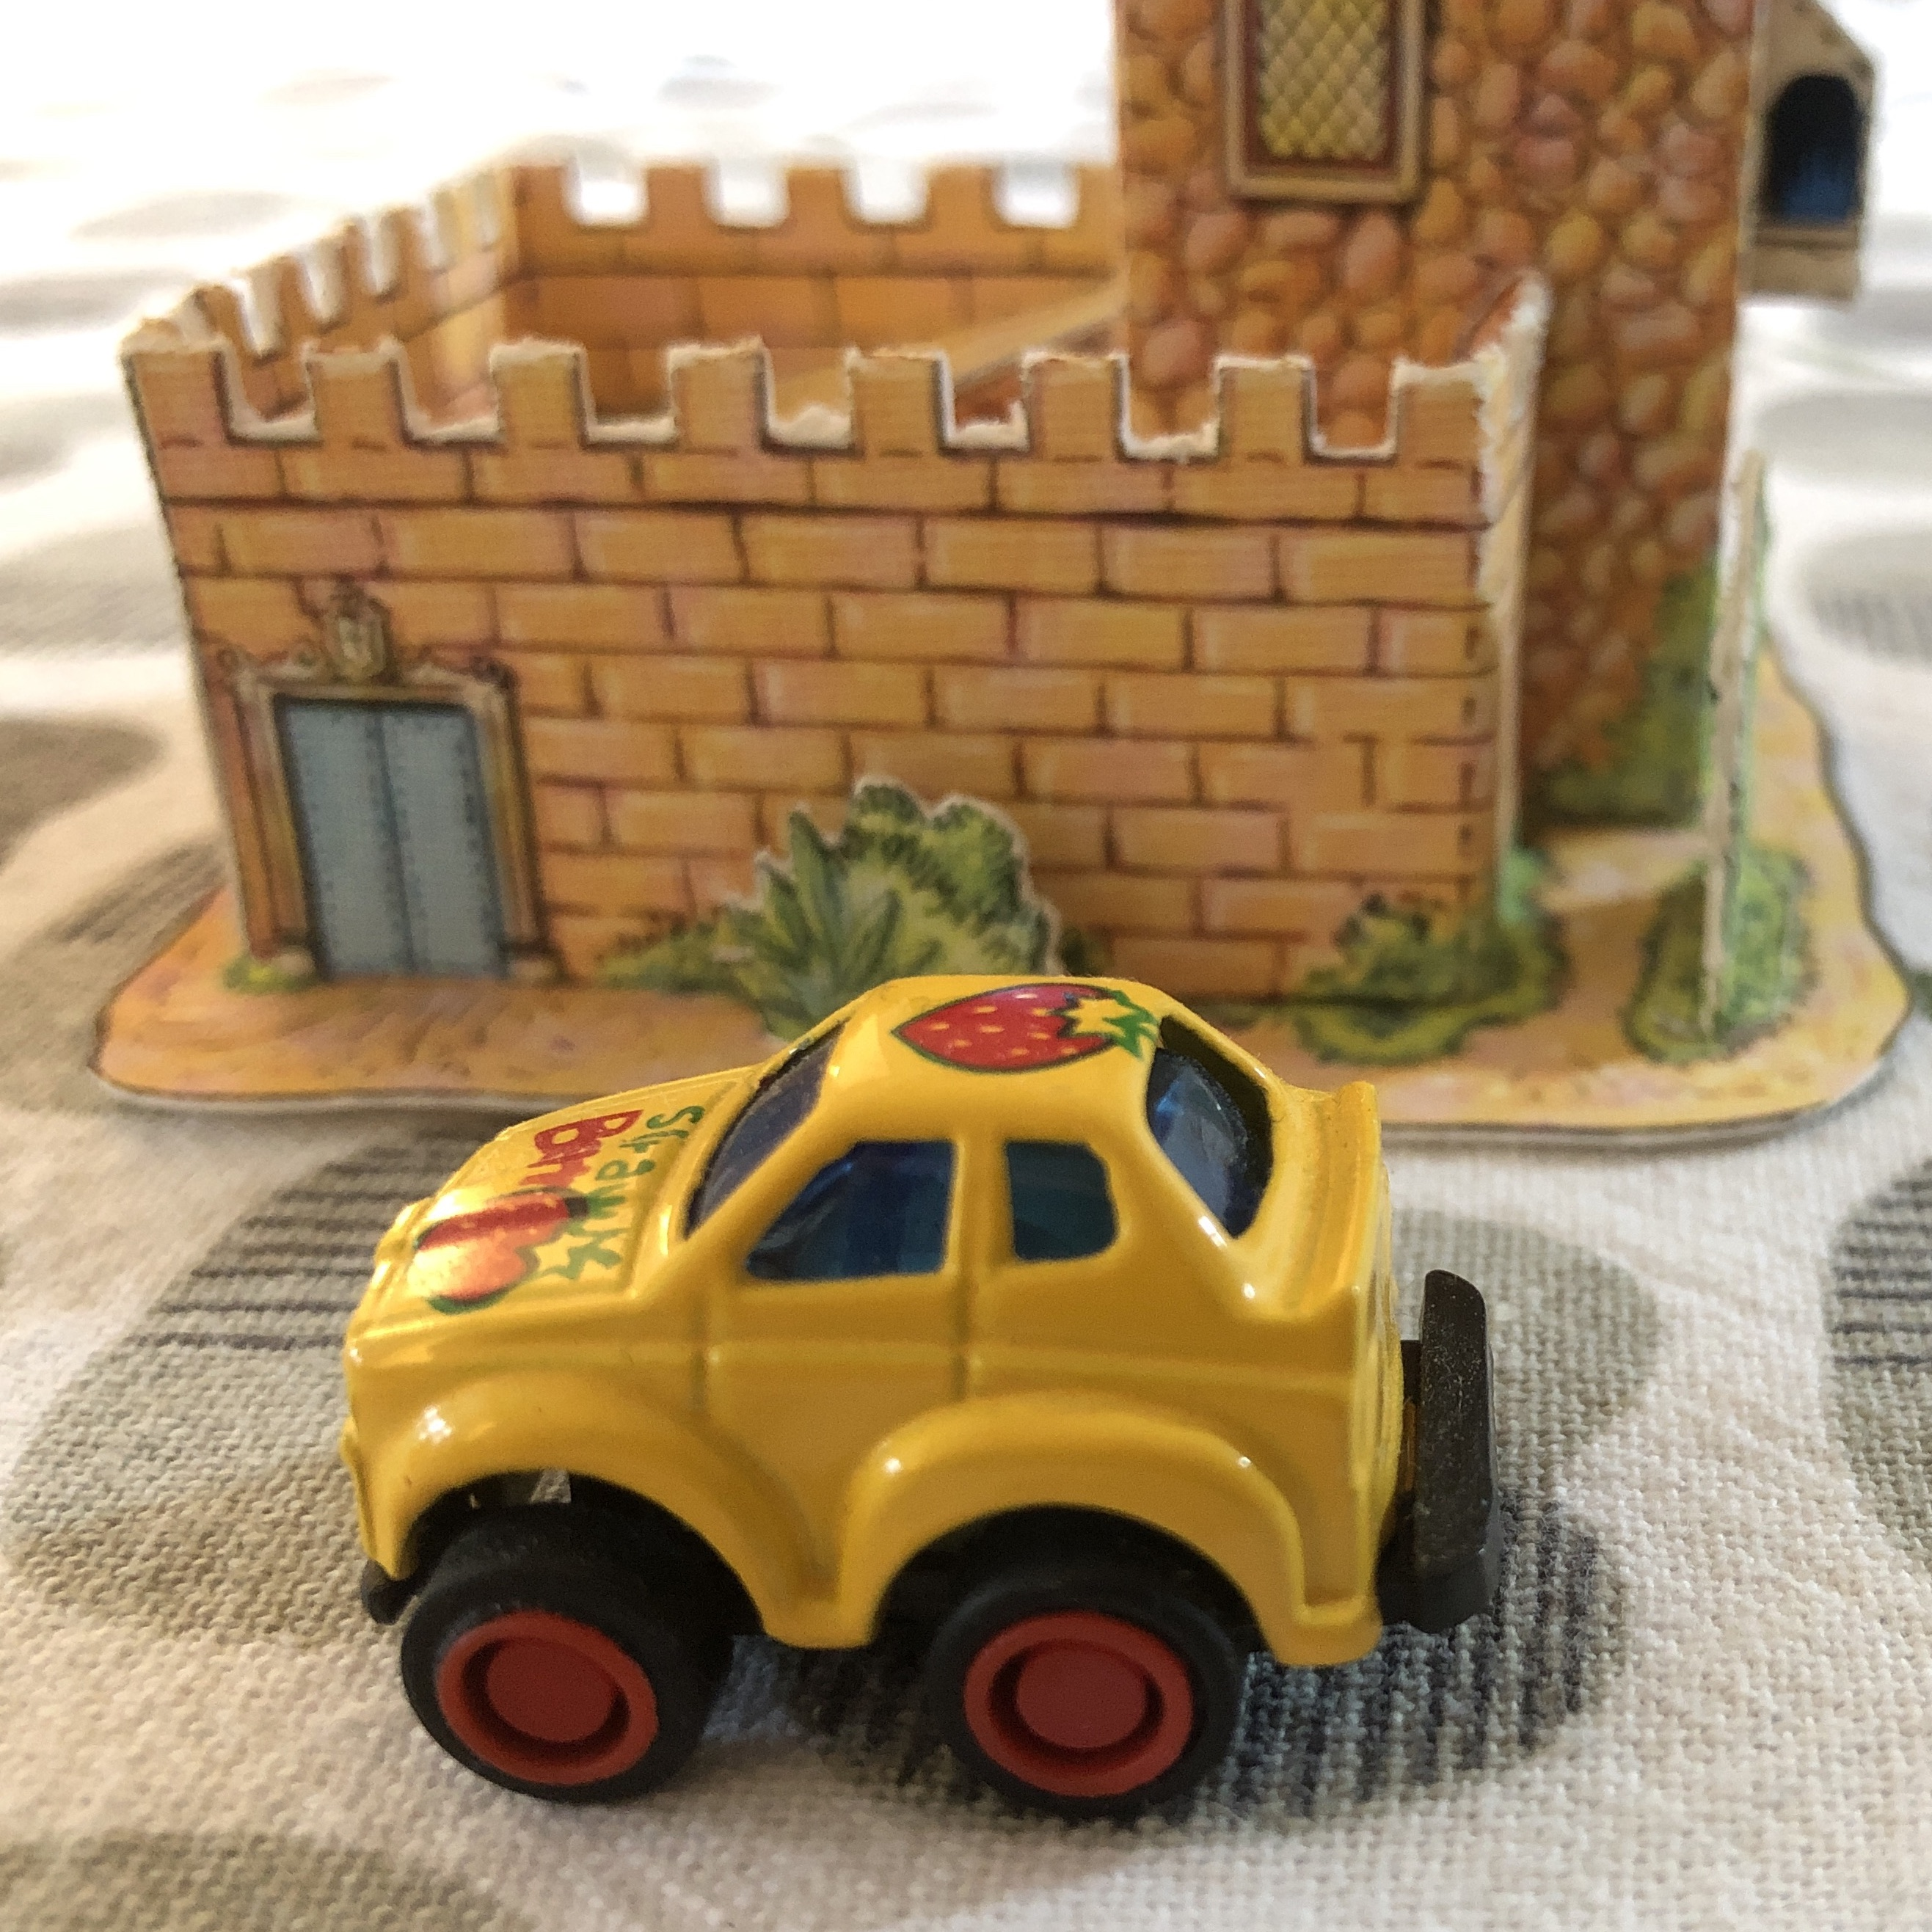
\includegraphics[width=0.32\linewidth]{figures/object_recognition/IMG_4467.jpeg}
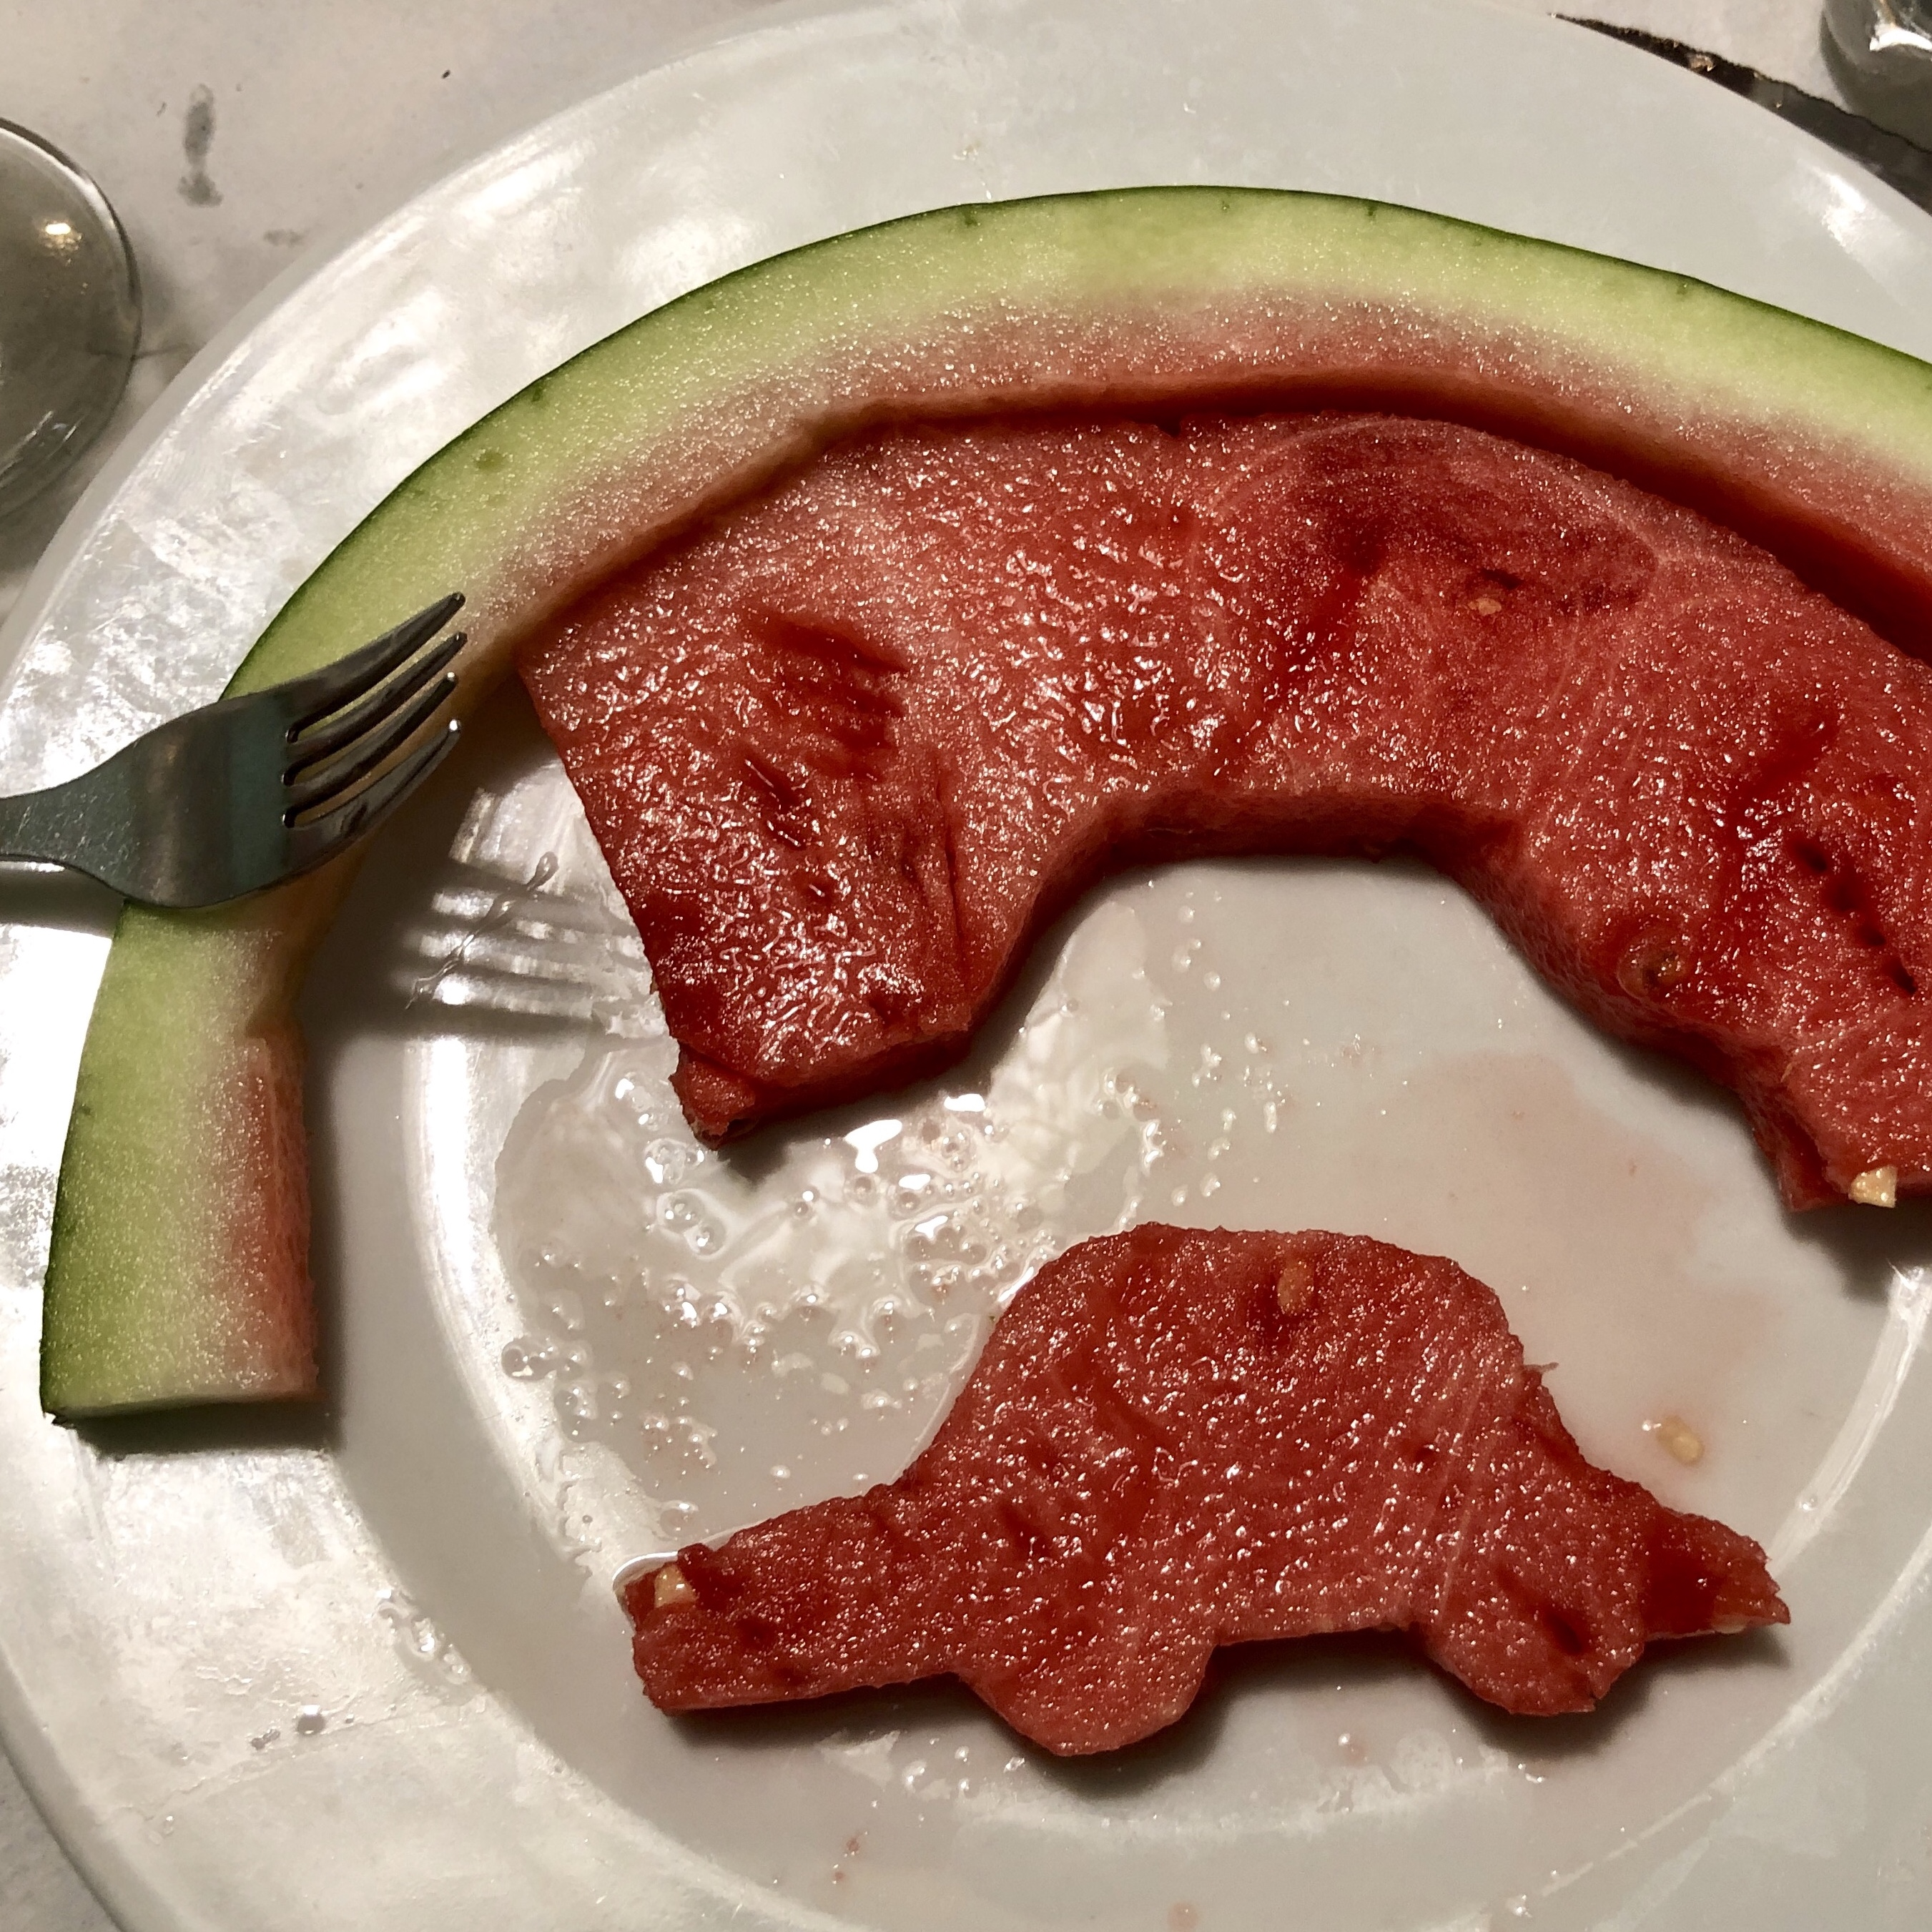
\includegraphics[width=0.32\linewidth]{figures/object_recognition/IMG_9325.jpeg}
}
\caption{Which of these images contains a car? This is a simple question that does not have a simple answer.}
\label{fig:whatisacar}
\end{figure}

Which of this images of \fig{\ref{fig:whatisacar}} contains a car? A simple question that does not have a simple answer. The top three images contain cars, although with increasing difficulty. However, for the three images on the second row, it is not clear what the desired answer it is. We can clearly recognize the content of those images, but it feels as if using a single word for describing those images leaves too much ambiguity. Is a car under construction already a car? Is the toy car a car? And if we play with food and make a car out of watermelon, would that be a car? Probably not. But if a vision system classifies that shape as a car, would that be a mistake like any other? 

Although it is not clearly stated in the problem definition, language plays a big role in object classification. The objects in \fig{\ref{fig:object_recognition_pepper}} are easily recognizable to us, but if we ask the question "Is there a fruit in this picture?," the answer is a bit more complex than it might appear on a first glance.

%I am sure you recognize the objects in the image bellow, but if I ask the question {\em Is there any fruit on this picture?} the answer is a bit more complex than it might appear on a first glance. 

%\vspace{-.2in}
\begin{figure}[h]
\centerline{
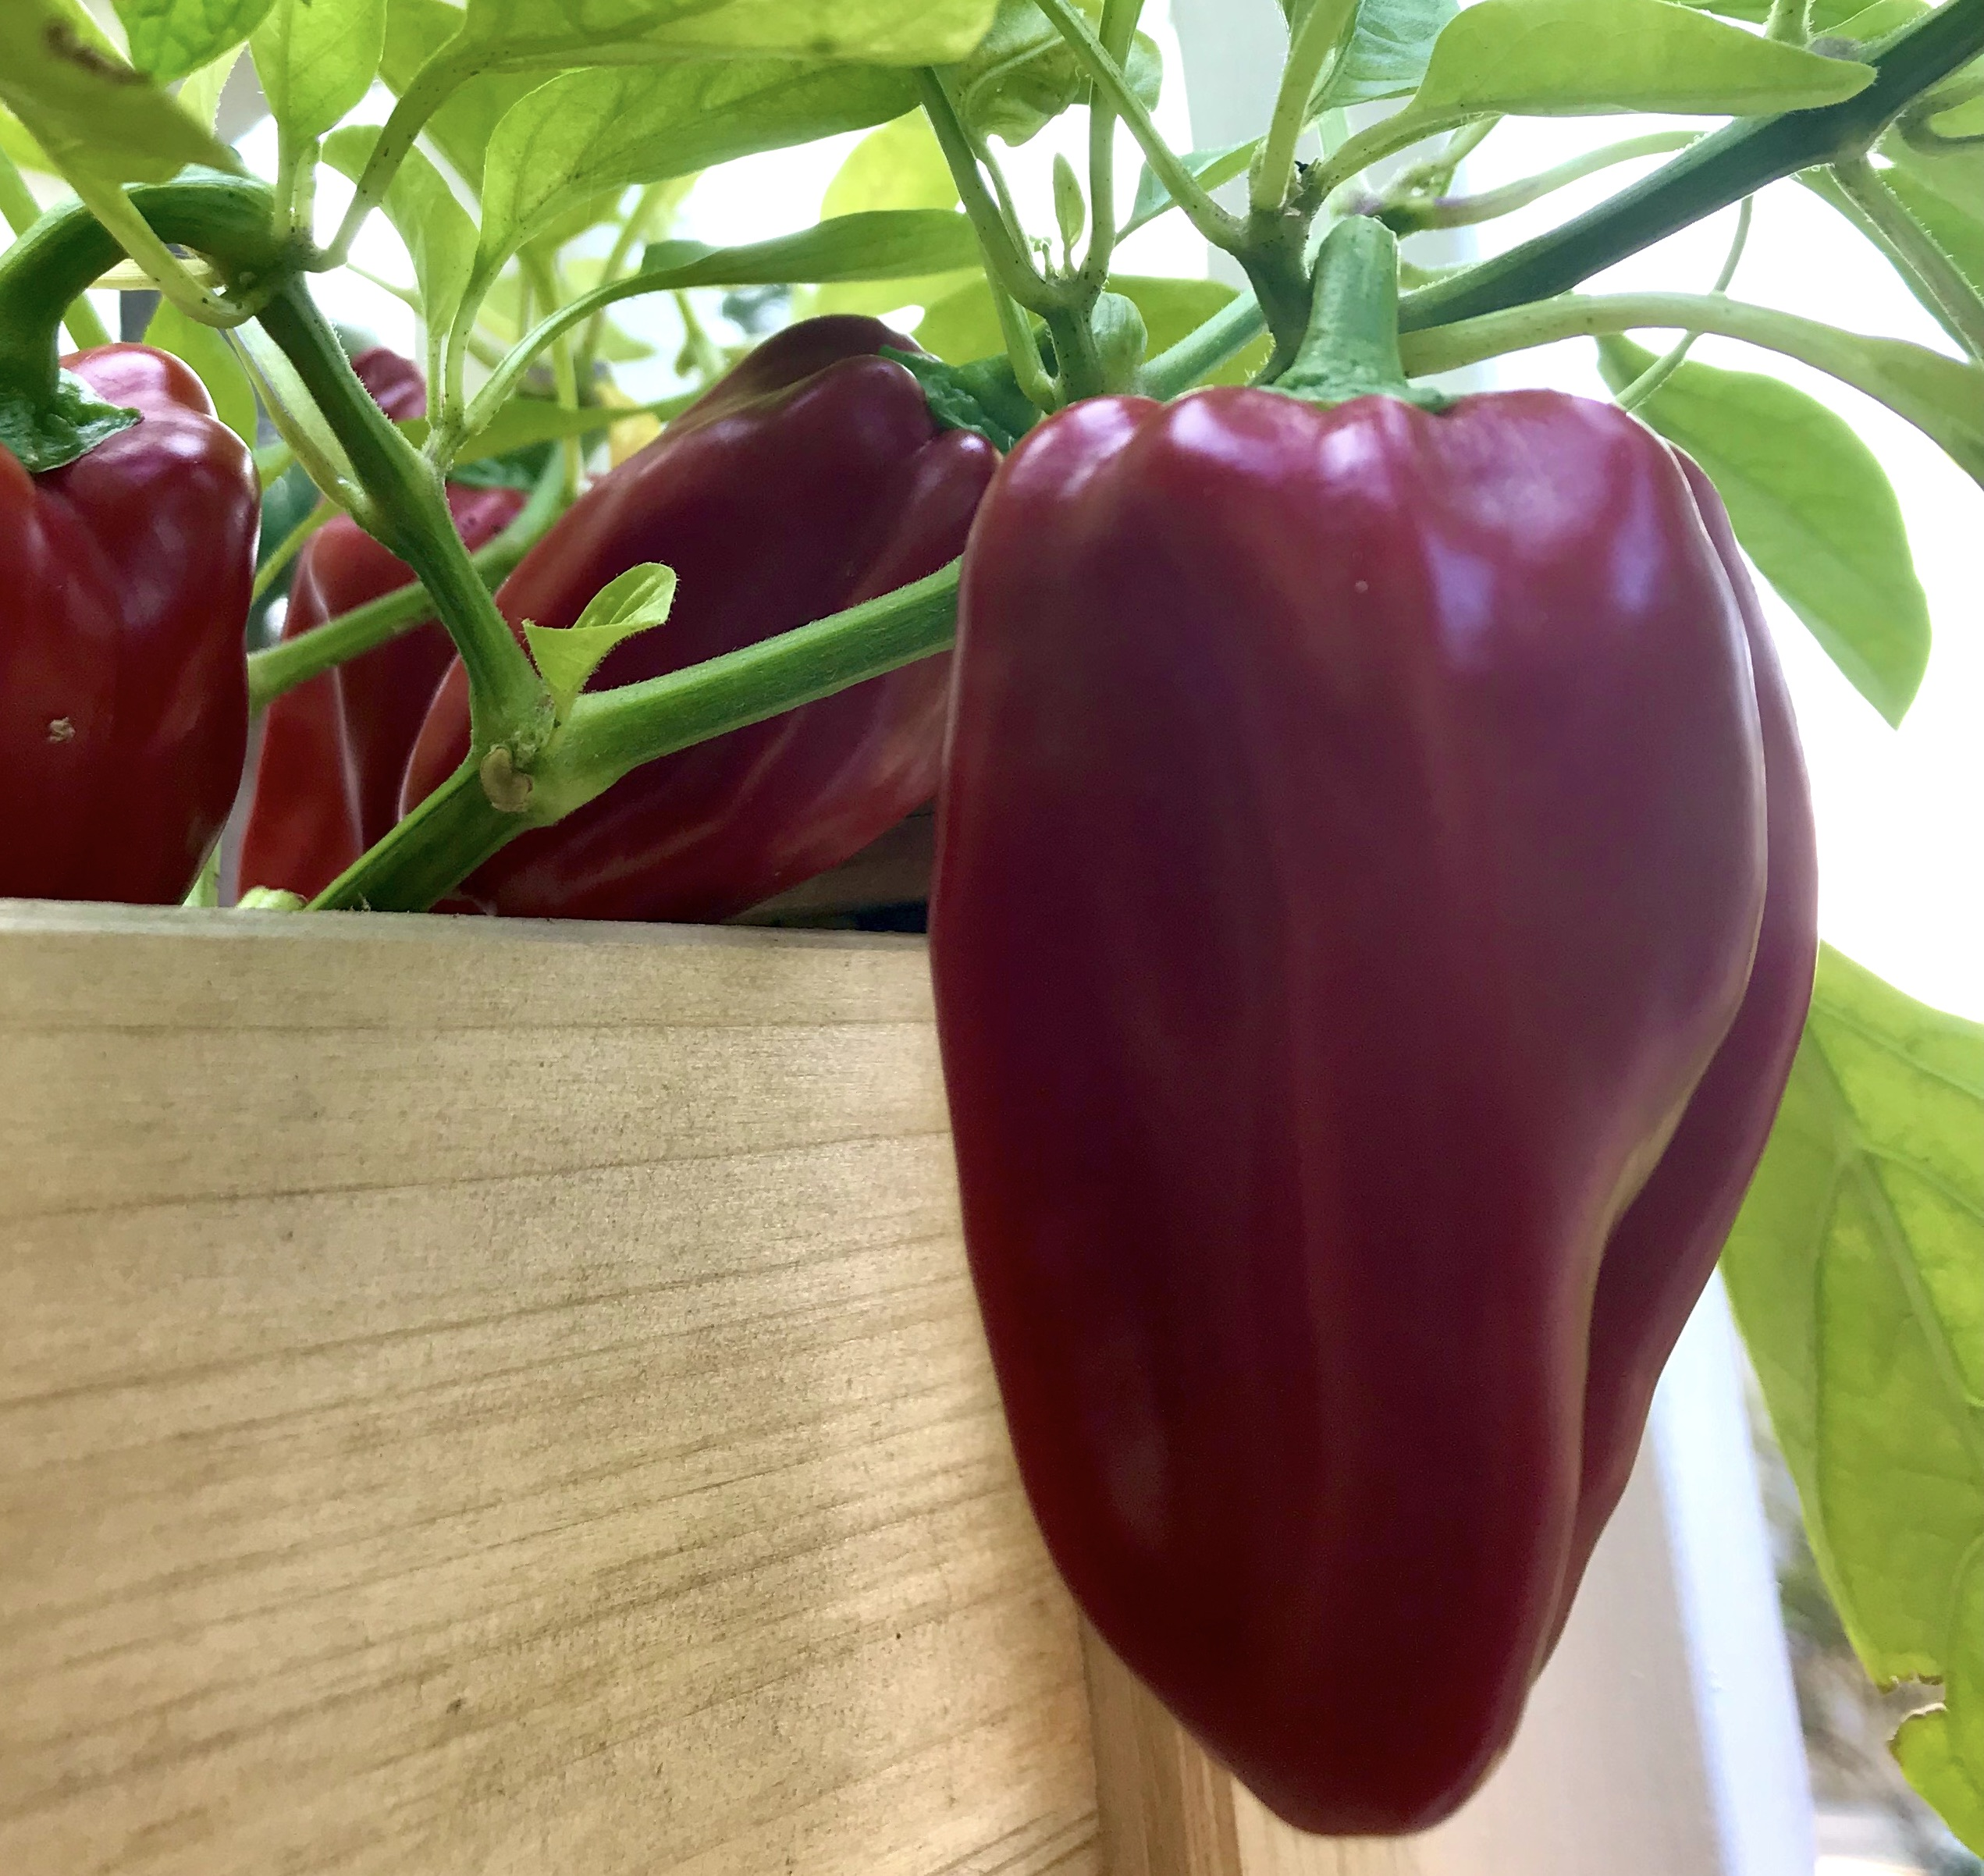
\includegraphics[width=0.32\linewidth]{figures/object_recognition/pepper.jpg}
}
\caption{A pepper is a fruit according to botanics, and it is a vegetable according to the culinary classification.}
\label{fig:object_recognition_pepper}
\end{figure}
%\vspace{-.2in}

What if the object is present in the scene but invisible in the image? What if there are infinite classes? In our formulation, $\hat {\bf y}$ is a vector of a fixed length. Therefore, we can only answer the question ``is object class $c$ present in the image?'' for a finite set of classes. What if we want to be able to answer an infinite set of questions? The next sections introduce more sophisticated formulations of object recognition that address some of these questions.


Is it possible to classify an image without localizing the object? How can we answer  the question ``Is object class $c$ present in the image?'' without localizing the object? One possibility is that the function $f$ has learned to localize the object internally but the information about the location is not being recorded in the output. Another possibility is that the function has learned to use other cues present in the image (biases in the dataset). As it is not trying to localize an object, the function $f$ will not get penalized if it uses shortcuts such as only recognizing one part of the object (e.g., such as the head of a dog, or car wheels), or if it makes use of contextual biases in the dataset (e.g., all images with grass and blue skies have horses, or all streets have cars) or detects unintended correlations between low-level image properties and the image content (e.g., all images of insects have a blurry background). As a consequence, image classification performance could mislead us into believing that the classifier works well and that it has learned a good representation of the object class it classifies. 

%Same or different
%- deals with an infinite number of classes.

%$y = f(x_1,x_2)$

%We will discuss bias on societal impacts on chapter XX.

\section{Object Localization}

For many applications, saying that an object is present in the image is not enough. Suppose that you are building a visual system for an autonomous vehicle. If the visual system only tells the navigation system that there is a person in the image it will be insufficient for deciding what to do. Object localization consists of localizing where the object is in the image. There are many ways one can specify where the object is. The most traditional way of representing the object location is using a {\bf bounding box} (\fig{\ref{fig:object_detection_bb}}), that is, finding the image-coordinates of a tight box around each of the instances of class $c$ in the image $\bf x$.



%FIGURE: show bounding boxes for some classes. 

\subsection{Formulation}

How you look at an object does not change the object itself (whether you see it or feel it, etc.). This induces translation and scale invariance. Let's build a system that has this property. 

We will formulate object detection as a function that maps the input image ${\bf x}$ into a list of bounding boxes $\hat {\bf b}_i$ and the associated classes to each bounding box encoded by a vector $\hat {\bf y}_i$. 
%\marginnote{
\begin{figure}[h]
\centerline{
\includegraphics[width=0.4\linewidth]{figures/object_recognition/object_detection_bb.eps}
}
\caption{Car localization using bounding boxes. Each instance is shown with a different color.}
\label{fig:object_detection_bb}
\end{figure}
%}


The class vector, $\hat {\bf y}_i$, has the same structure as in the image classification task but now it is applied to describe each bounding box. Bounding boxes are usually represented as a vector of length 4 using the coordinates of the two corners, ${\bf b} = \left[ x_1, y_1, x_2, y_2 \right]$, or with the center coordinates, width, and height, ${\bf b} = \left[ x_c, y_c, w, h \right]$. 
Our goal is a function $f$ that outputs a set of bounding boxes, $\mathbf{b}$, and their classes $\mathbf{y}$:
\begin{equation}
\{\hat {\bf y}_i, \hat {\bf b}_i\} = f({\bf x})
\end{equation}

Most approaches for object detection have three main steps. In the first step, a set of candidate bounding boxes are proposed. In the second step, we loop over all proposed bounding boxes, and for each one, we apply an classifier the image patch inside the bounding box. In the third and final step, the selected bounding boxes are postprocessed to remove any redundant detections. 

\subsubsection{Window scanning approach}
%~\\
%{\bf Window scanning approach}. 
In its simplest form, the problem of object localization is posed as a binary classification task, namely distinguishing between a single object class and background class. Such a classification task can be turned into a detector by sliding it across the image (or image pyramid), and classifying each local window as shown in \fig{\ref{fig:scanningWindow2}}.

%\vspace{-.2in}
\begin{figure}[h]
\centerline{
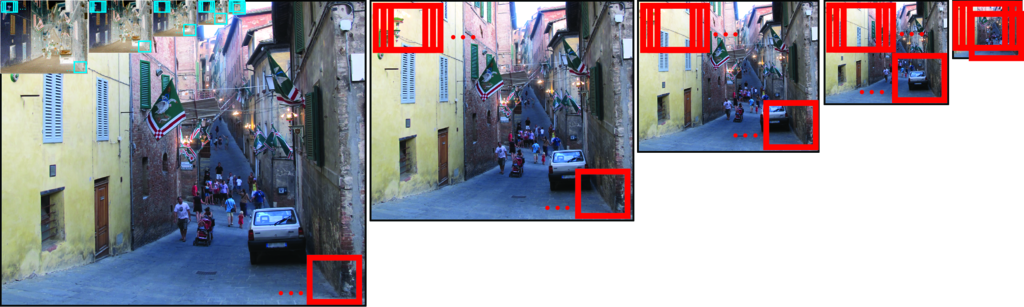
\includegraphics[width=1\linewidth]{figures/object_recognition/scanningWindow2.eps}
}
\caption{Window scanning approach using a multiscale image pyramid.}
\label{fig:scanningWindow2}
\end{figure}
%\vspace{-.2in}

The algorithm is then simply:
\begin{algorithm}[h]
\SetAlgoVlined
\DontPrintSemicolon
\marginnote{{\bf Algorithm \ref{alg:scanning_window}}: Scanning window approach for object localization.}
\caption{Scanning window approach}
\faketablecaption{}
\label{alg:scanning_window}
%\begin{algorithm}[h!]
%\SetAlgoVlined
%\DontPrintSemicolon
{\bf Input:} Image;
{\bf Output:} Object bounding boxes and classes, $\{\hat{\mathbf{b}}_i, \hat{\mathbf{y}}_i\}_{i=1}^B$\;
$\{\hat{\mathbf{b}}_i\}_{i=1}^{B^{\prime}} \leftarrow$ list all bounding boxes (all locations, scales, aspect ratios, ...)\;

\For{\upshape $i= 1, \dots, B'$}{
    $\hat{\mathbf{y}}_i \leftarrow$ Classification of content in box $\hat{\mathbf{b}}_i$\;
}
$\{\hat{\mathbf{b}}_i, \hat{\mathbf{y}}_i\}_{i=1}^B \leftarrow$ Thresholding and non maximum suppression\;
\label{alg:object_localization}
\end{algorithm}

In this approach, location and translation invariance are achieved by the bounding box proposal mechanism. We can add another invariance, such as rotation invariance, by proposing rotated bounding boxes. 

\subsubsection{Selective search}
%~\\
The window scanning approach can be slow as the same classifier needs to be applied to tens of thousands of image patches. Selective search makes the process more efficient by proposing an initial set of bounding boxes that are good candidates to contain an object (\fig{\ref{fig:selective_search_pipeline}}). This proposal mechanism is performed by a selection mechanism simpler than the object classifier. 
This approach was motivated by the strategy used by the visual system in which attention is first directed toward image regions likely to contain the target \cite{wolfe2007,TreismanGelade1980,Koch_Ullman_1985}. This first attentional mechanism is very fast but might be wrong. Therefore, a second, more accurate but also more expensive, processing stage is required in order to take a reliable decision.  The advantage of this {\bf cascade} of decisions is that the most expensive classifier is only applied to a sparse set of locations (the ones selected by the cheap attentional mechanism) dramatically reducing the overall computational cost. The algorithm for selective search only differs from the window scanning approach on how the list of candidate bounding boxes is generated. Some approaches also add a bounding box refinement step.
The overall approach is described in \algref{\ref{alg:selective_search}}.

%\marginnote{
\begin{figure}[t]
\centerline{
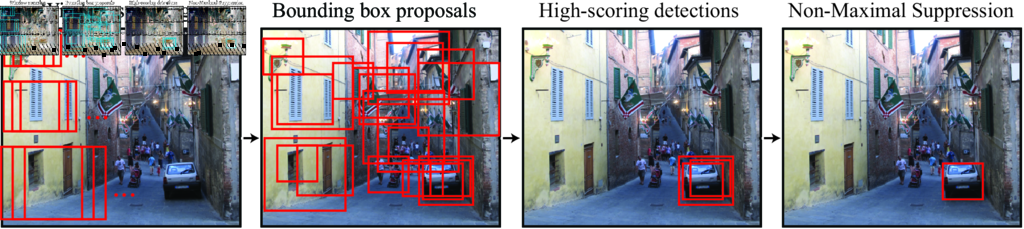
\includegraphics[width=1\linewidth]{figures/object_recognition/selective_search.eps}
}
\caption{A first classifier selects candidate bounding boxes. A second, stronger, classifier makes the final detections (e.g., cars). Non maximum suppression (NMS) removes overlapping detections.}
\label{fig:selective_search_pipeline}
\end{figure}
%}


\begin{algorithm}[h]
\SetAlgoVlined
\DontPrintSemicolon
\marginnote{{\bf Algorithm \ref{alg:selective_search}}: Selective search approach for object localization.}
\caption{Selective search}
\faketablecaption{}
\label{alg:selective_search}
{\bf Input:} Image;
{\bf Output:} Object bounding boxes and classes, $\{\hat{\mathbf{b}}_i, \hat{\mathbf{y}}_i\}_{i=1}^B$\;
$\{\hat{\mathbf{b}}_i\}_{i=1}^{B^{\prime}} \leftarrow$ Bounding box proposals\;

\For{\upshape $i= 1, \dots, B$}{
    $\hat{\mathbf{y}}_i \leftarrow$ Classification of content in box $\hat{\mathbf{b}}_i$\;
    $\hat{\mathbf{b}}_i \leftarrow$ Bounding box refinement\;
}
$\{\hat{\mathbf{b}}_i, \hat{\mathbf{y}}_i\}_{i=1}^B \leftarrow$ Thresholding and non-maximum suppression\;
\end{algorithm}

\marginnote{The non maximum suppression algorithm takes as input a set of object bounding boxes and confidences, $S=\{\hat{\mathbf{b}}_i, \hat{\mathbf{y}}_i\}_{i=1}^B$\. Then, it proceeds with the following iteration: 
(1) Take the highest confidence bounding box from the set $S$ and add it to the final set $S^*$.
(2) Remove from $S$ the selected bounding box and all the bounding boxes with an IoU larger than a threshold.
(3) go to step 1 until $S$ is empty.}[-2.2in]

This algorithm has four main steps. In the first step, the algorithm uses an efficient window scanning approach to produce a set of candidate bounding boxes. In the second step, we loop over all the candidate bounding boxes, we crop out the box and resize it to a canonical size, and then we apply an object classifier to classify the cropped image as containing the object we are looking for or not. In the third step, we refine the bounding box for the crops that are classified as containing the object. And finally, in the fourth step, we remove low-scoring boxes and we use {\bf non maximum suppression} (NMS) to discard overlapping detections likely to correspond to the same object, so as to output only one bounding box for each instance present in the image. Each step can be implemented in several different ways, giving rise to different approaches. The whole pipeline is summarized in \fig{\ref{fig:selective_search_pipeline}}.

Bounding box proposal (represented as $f_0$ in the diagram bellow) can be implemented in several ways (e.g., using image segmentation \cite{Uijlings2013}, a neural network \cite{Ren2015}, or a window scanning approach with a low-cost classifier). The classification and bounding box refinement, $f_1$, can be implemented by a classifier and a regression function.
%\vspace{-.1in}
\begin{figure}
\centerline{
\includegraphics[width=.4\linewidth]{figures/object_recognition/selective_search_architecture.eps}
}
\caption{Sketch of the selective search architecture. The image is first broken into candidate regions. Then each region is processed individually using a classifier and a regression.}
\end{figure}
%\vspace{-.2in}


% Relate the definition to the measure of performance

% Object detection: Search and classification
% 		Scanning window -> pyramids
% 		Selective search

\subsubsection{Cascade of classifiers}
%~\\
Trying to localize an object in an image is like finding a needle in a haystack: the object is usually small and might be surrounded by a complex background. 
%Detecting an object on an image using classifiers requires applying a very selective classification function at all possible locations and scales in the image. 
Selective search reduced the complexity of the search by dividing the search in two steps: a first, fast, and cheap classification function that detects good candidate locations; and a second, slow, and expensive classification function capable of accurately classifying the object and that only needs to be applied in a subset of all possible locations and scales. Cascade of classifiers pushes this idea to the limit by dividing the search in a sequence of classifiers of increasing computational complexity and accuracy. 


The algorithm for the cascade of classifiers is:

\begin{algorithm}[h]
\SetAlgoVlined
\DontPrintSemicolon
\marginnote{{\bf Algorithm \ref{alg:cascade_classifier}}: Cascade of classifiers for object localization.}
\caption{Cascade of classifiers}
\faketablecaption{}
\label{alg:cascade_classifier}
{\bf Input:} Image, $\mathbf{x}$;
{\bf Output:} Object bounding boxes and classes, $\{\hat{\mathbf{b}}_i, \hat{\mathbf{y}}_i\}_{i=1}^B$\;

$S_0 = \{\hat{\mathbf{b}}_i\}_{i=1}^{B_0} \leftarrow$ Initial set of bounding box proposals\;

\For{\upshape $j = 1, \dots, \text{Levels}$}{

\For{\upshape $\mathbf{b}_i \in S_{j-1}$}{
    %$(\hat{\mathbf{b}}_i, \hat{\mathbf{y}}_i) = f_j(\mathbf{x}, \mathbf{b}_i) \leftarrow$ Classification of content in box $\hat{\mathbf{b}}_i$ \;
    $\hat{\mathbf{y}}_i = f_j(\mathbf{x}, \hat{\mathbf{b}}_i) \leftarrow$ Classification of content in box $\hat{\mathbf{b}}_i$ \;
    %$\hat{\mathbf{y}}_i \leftarrow$ Classification of content in box $\hat{\mathbf{b}}_i$\;
    %$\hat{\mathbf{b}}_i \leftarrow$ Bounding box refinement\;
}
$S_{j} = \{ \hat{\mathbf{b}}_i  \text{ such that } \hat{\mathbf{y}}_i > \theta_j \} \leftarrow$ Keep high scoring bounding boxes\;
}
$\{\hat{\mathbf{b}}_i, \hat{\mathbf{y}}_i\}_{i=1}^B \leftarrow$ Non maximum suppression\;
\end{algorithm}

Cascades of classifiers became popular in computer vision when Paul Viola and Michael Jones \cite{Viola01} introduced it in 2001 with a ground-breaking real-time face detector based on a cascade of boosted classifiers. In parallel, Fleuret and Geman \cite{Fleuret2001} also proposed a system that performs a sequence of binary tests at each location. Each binary test checks for the presence of a particular image feature. Early versions of this strategy were also inspired by the game ``Twenty Questions''  \cite{Geman1994}. 

In a cascade, computational power is allocated into the image regions that are more likely to contain the target object while regions that are flat or contain few features are rejected quickly and almost no computations are allocated in them. The following figure, from \cite{Fleuret2001}, shows a beautiful illustration of how a cascaded classifier allocates computing power in the image when trained to detect faces. The intensity shown in the heat map is proportional to the number of levels in the cascade applied to each location.

%\vspace{-.1in}
\begin{figure}
\centerline{
\includegraphics[width=.8\linewidth]{figures/object_recognition/cascade.eps}
}
\caption{(left) input image with the output of a face detector from 1999. (right) The heat map reports the computational cost at each location. Most of the computation was allocatted into the wrong detections in the top left corner. Figure from \cite{Fleuret2001}.}
\end{figure}
%\vspace{-.1in}

It is interesting to point out that the scanning window approach ($Levels = 1$) and the selective search procedure ($Levels = 2$) are special cases of this algorithm. The cascade of classifiers usually does not have a bounding box refinement stage as it already started with a full list of all bounding boxes, but it could be added if we wanted to add new transformations not available in the initial set (e.g., rotations). 

\subsubsection{Other approaches}
%~\\
Object localization is an active area of research and there are a number of different formulations that share some elements with the approaches we shared previously. One example is YOLO \cite{Redmon2016}, which makes predictions by looking at the image globally. It is not as accurate as some of the scanning methods but it can be computationally more efficient. There are many other approaches that we will not summarize here as the list will be obsolete shortly. Instead, we will continue focusing on general concepts that should help the reader understand other approaches.

\subsection{Object Localization Loss}

The object localization loss has to take into account two complementary tasks: classification and localization.
\begin{itemize}
\item Classification loss ($\mathcal{L}_{\text{cls}}$): For each detected bounding box, does the predicted label matches the ground truth at that location? 
\item Localization loss ($\mathcal{L}_{\text{loc}}$): How close is the detected location to the ground truth object location?
\end{itemize}

For each image, the output of our object detector is a set of bounding boxes $\{\hat{\mathbf{b}}_i, \hat{\mathbf{y}}_i\}_{i=1}^B$, where $B$ is likely to be larger than the number of ground truth bounding boxes in the training set. The first step in the evaluation is to associate each detection with a ground truth label so that we have a set $\{\mathbf{b}_i, \mathbf{y}_i\}_{i=1}^B$. For each of the predicted bounding boxes that overlaps with the ground truth instances, we want to optimize the system parameters to improve the predicted locations and labels. The remaining predicted bounding boxes that do not overlap with ground truth instances are assigned to the background class, $\mathbf{y}_i=0$. For those bounding boxes, we want to optimize the model parameters in order to reduce their predicted class score, $\hat{\mathbf{y}}_i$. This process is illustrated in the following figure. The detector produces a set of bounding boxes for candidate car locations. Those are compared with the ground truth data. Each detected bounding box is assigned one ground truth label (indicated by the color) or assigned to the background class (indicated in white). Note that several detections can be assigned to the same ground truth bounding box. 

%\vspace{-.2in}
\begin{figure}
\centerline{
\includegraphics[width=1\linewidth]{figures/object_recognition/detections.eps}
}
\caption{%For evaluation, we need to assign detected bounding boxes with ground-truth annotations. 
(left) Detector output (using a low threshold to generate many detections). (middle) ground truth bounding boxes (one color per instance). (right) Detector outputs that overlap with ground-truth annotations, which are color coded.}
\end{figure}
%\vspace{-.2in}

Now that we have assigned detections to ground truth annotations, we can compare them to measure the loss. For the classification loss, as each bounding box can only have one class, we can use the cross-entropy loss: 
\begin{equation}
    \mathcal{L}_{\text{cls}}(\hat{\mathbf{y}}_i, \mathbf{y}_i)
     = -  \sum_{c=1}^{K} y_{c,i} \log(\hat{y}_{c,i}) 
\end{equation}
where $K$ is the number of classes.  

Let's now focus on the second part; how do we measure the localization loss $\mathcal{L}_{\text{loc}} (\hat{\mathbf{b}}_i, \mathbf{b}_i)$? One typical measure of similarity between two bounding boxes is the {\bf Intersection over Union} (IoU) as shown in the following drawing:

%\vspace{-.1in}
\begin{figure}
\centerline{
\includegraphics[width=0.5\linewidth]{figures/object_recognition/iou.eps}
}
\caption{Sketch of the computation of intersection over union for two bounding boxes.}
\end{figure}
%\vspace{-.2in}

The IoU is a quantity between 0 and 1, with 0 meaning no overlap and 1 meaning that both bounding boxes are identical. As the IoU is a similarity measure, the loss is defined as:
\begin{equation}
\mathcal{L}_{\text{loc}} (\hat{\mathbf{b}}, \mathbf{b})= 1-IoU (\hat{\mathbf{b}}, \mathbf{b}).
\end{equation}
The IoU is translation and scale invariant, and it is frequently used to evaluate object detectors. A simpler loss to optimize is the L2 regression loss:
\begin{equation}
\mathcal{L}_{\text{loc}} (\hat{\mathbf{b}}, \mathbf{b}) = (\hat{x}_1 - x_1)^2 + (\hat{x}_2 - x_2)^2 + (\hat{y}_1 - y_1)^2 + (\hat{y}_2 - y_2)^2
\end{equation}
The L2 regression loss is translation invariant, but it is not scale invariant. The L2 loss is larger for big bounding boxes. The next graph (\fig{\ref{fig:iou_l2_comparison}}) compares the IoU loss, and the L2 regression loss for two square bounding boxes, with an area equal to 1, as a function of the relative $x$-displacement.

%\vspace{-.2in}
\begin{figure}
\centerline{
\includegraphics[width=1\linewidth]{figures/object_recognition/iou_l2_comparison.eps}
}
\caption{Comparison of the the IoU loss and the L2 regression loss for two square bounding boxes as a function of the relative $x$-displacement.}
\label{fig:iou_l2_comparison}
\end{figure}
%\vspace{-.2in}

The IoU loss becomes 1 when the two bounding boxes do not overlap, which means that there will be no gradient information when running backpropagation. 

Now we can put together the classification and the localization loss to compute the overall loss:
%% A nice description here: https://arxiv.org/pdf/1312.2249.pdf
\begin{equation}
    \mathcal{L}( \{\hat{\mathbf{b}}_i, \hat{\mathbf{y}}_i\}, \{\mathbf{b}_i, \mathbf{y}_i\})
     =  \mathcal{L}_{\text{cls}}(\hat{\mathbf{y}}_i, \mathbf{y}_i) +
     \lambda \mathbbm{1} (\mathbf{y}_i \neq 0)
     \mathcal{L}_{\text{loc}} 
     (\hat{\mathbf{b}}_i, \mathbf{b}_i)
\end{equation}
where the indicator function $\mathbbm{1} (\mathbf{y}_i \neq 0)$ sets to zero the location loss for the bounding boxes that do not overlap with any of the ground-truth bounding boxes. The parameter $\lambda$ can be used to balance the relative strength of both losses. This loss makes possible to train the whole detection algorithm end-to-end. It is possible to train the localization and the classification stages independently and some approaches follow that strategy. 


%\subsection{Architecture}

\subsection{Evaluation}

There are several ways of evaluating object localization approaches. The most common approach is measuring the average precision-recall. 

Just as we did when defining the localization loss, we need to assign detection outputs to ground truth labels. We can do this in several ways and they can result in different measures of performance. The methodology introduced in the PASCAL challenge used the following procedure. 

{\bf Assign detections to ground truth labels}: For each image, sort all the detections by their score, $\hat{\mathbf{y}}_i$. Then, loop over the sorted list in decreasing order. For each bounding box, compute the IoU with all the ground truth bounding boxes. Select the ground truth bounding box with the highest IoU. If the IoU is larger than a predefined threshold, (a typical value is 0.5) mark the detection as correct and remove the ground truth bounding box from the list to avoid double counting the same object. If the IoU is below the threshold, mark the detection as incorrect and do not remove the ground truth label. Repeat this operation until there are no more detections to evaluate. 

{\bf Precision-recall curve} measures the performance of the detection as a function of the decision threshold. As each bounding box comes with a confidence score $\hat{\mathbf{y}}_i$, we need to use a threshold, $\beta$, to decide if an object is present at the bounding box location $\hat{\mathbf{b}}_i$ or not. Given a threshold $\beta$, the number of detections is $\sum_i  \mathbbm{1} (\hat{\mathbf{y}}_i > \beta)$ and the number of correct detections is $\sum_i  \mathbbm{1} (\hat{\mathbf{y}}_i > \beta) \times \mathbf{y}_i$. From these two quantities we compute the {\bf precision} as the percentage of correct detections:

%CD (\beta) =  \sum_i  \mathbbm{1} (\hat{\mathbf{y}}_i > \beta) \mathbf{y}_i
%MD (\beta)

\begin{equation}
Precision(\beta) = \frac{\sum_i  \mathbbm{1} (\hat{\mathbf{y}}_i > \beta) \times \mathbf{y}_i} {\sum_i  \mathbbm{1} (\hat{\mathbf{y}}_i > \beta)}
\end{equation}

The precision only gives a partial view on the detector performance as it does not account for the number of ground truth instances that are not detected (misdetections). The {\bf recall} measures the proportion of ground truth instances that are detected for a given decision threshold $\beta$:
\begin{equation}
Recall (\beta) = \frac{\sum_i  \mathbbm{1} (\hat{\mathbf{y}}_i > \beta) \times \mathbf{y}_i} {\sum_i \mathbf{y}_i}
\end{equation}

Both, the precision and recall, are quantities between 0 and 1. High values of precision and recall correspond to high performance. The next graph (\fig{\ref{fig:example_precision_recall}}) shows the precision-recall curve as a function of $\beta$ (decision threshold).


%\vspace{-.1in}
\begin{figure}
\centerline{
\includegraphics[width=.4\linewidth]{figures/object_recognition/example_precision_recall.eps}
}
\caption{Example of a precision-recall curve. This is a standard plot to evaluate detection algorithms. It is usually summarized by the area under the curve. In this example, note that recall stops around 0.5. This is because this algorithm fails to detect the other 50 percent of the test examples for all thresholds $\beta$.}
\label{fig:example_precision_recall}
\end{figure}
%\vspace{-.2in}
The precision-recall curve is non-monotonic. The average precision (AP) summarizes the entire curve with one number. The AP is the area under the precision-recall curve, and it is a number between 0 and 1.

% 2-take highest scoring bounding box
% 3-compute IoU with all the ground truth bounding boxes.
% 4-if IoU > threshold, mark the detection as correct and remove the
% groundtruth bounding box from the list of annotations so that the same
% object can not be detected twice. 
% 5-else; mark bounding box as incorrect.

%One of the simplest evaluation metrics is the ROC. 

%miss-detection, false alarm,

%Performance evaluation
% 		intersection over union. There are some  cool figures showing what IoU of 0.5 means, 0.7, 0.9, ... We could show this for bounding boxes and for segmentations  of dogs (or horses), showing examples of different segmentations and the associated measures. 

% 		precision-recall, ROC. Make a FIGURE  showing sets and what  each  measure represents. 

%average  precision  (AP), meanAP   (averaged across all categories)	
		
% But why is object classification different from detection?

\subsection{Shortcomings}

Bounding boxes can be very powerful in many applications. For instance, digital cameras detect faces and use bounding boxes to encode their location. The camera uses the pixels inside the bounding box to automatically set the focus and exposure time.

But using bounding boxes to represent the location objects will not be appropriate for objects with long and thin structures or for regions that do not have well-defined boundaries (\fig{\ref{fig:segmenting_trees}}). It is useful to differentiate between {\bf stuff} and {\bf objects}. Stuff refers to things that do not have well-defined boundaries such as grass, water, and sky (we already discussed this in \chap{\ref{chap:textures}}). But the distinction between stuff and objects is not very sharp. In some images, object instances might be easy to separate like the two trees in the left image below, or become a texture where instances cannot be detected individually (as shown in the right image). In cases with lots of instances, bounding boxes might not appropriate and it is better to represent the region as ``trees'' than to try to detect each instance.  

%\vspace{-.1in}
\begin{figure}
\centerline{
\includegraphics[width=1\linewidth]{figures/object_recognition/segmenting_trees.png}
}
\caption{Bounding boxes are not an appropriate representation of the location of trees. This is true for many object classes with extended shapes that are hard to approximate with a box.}
\label{fig:segmenting_trees}
\end{figure}
%\vspace{-.2in}

Even when there are few instances, bounding boxes can provide an ambiguous localization when two objects overlap because it might not be clear which pixels belong to each object. 

Bounding boxes are also an insufficient object description if the task is robot manipulation. A robot will need a more detailed description of the pose and shape of an object to interact with it. 

Let's face it, localizing objects with bounding boxes does not address most of the shortcomings present in the image classification formulation. In fact, it adds a few more.
		

\section{Class Segmentation}

An object is something localized in space. There are other things that are not localized such as fog, light, and so on. Not everything is well-described by a bounding box (stuff, wiry objects, etc.). Instead we can try to classify each pixel in an image with an object class. Per-pixel classification of object labels, illustrated in \fig{\ref{fig:semantic_class_segmentation}}, is referred to as {\bf semantic segmentation}.


%\vspace{-.2in}
\begin{figure}
\centerline{
\includegraphics[width=0.6\linewidth]{figures/object_recognition/semantic.eps}
}
\caption{Semantic segmentation. Every pixel is annotated with a semantic tag (red = car, blue = building, green = road, yellow = sidewalk and cyan = sign).}
\label{fig:semantic_class_segmentation}
\end{figure}
%\vspace{-.2in}

%$\mathbf{y} = f(\mathbf{x}, n, m)$ or as more 
In the most generic formulation, semantic segmentation takes an image as input, $\mathbf{x}(n,m)$, and it outputs a classification vector at each location $\mathbf{y}(n,m)$:
\begin{equation}
\hat{\mathbf{y}} \left[n,m \right] = f(\mathbf{x} \left[n,m \right])
\end{equation}

 
 
There are many ways in which such a function can be implemented. Generally the function $f$ is a neural network with an encoder-decoder structure (\fig{\ref{fig:segmentation_architecture}}), first introduced in \cite{Badrinarayanan2015}. 

%\vspace{-.2in}
\begin{figure}
\centerline{
\includegraphics[width=0.3\linewidth]{figures/object_recognition/segmentation_architecture.eps}
}
\caption{Sketch of the encoder-decoder architecture for semantic segmentation.}
\label{fig:segmentation_architecture}
\end{figure}
%\vspace{-.2in}

Another formulation consists of implementing a window-scanning approach where the function $f$ scans the image and takes as input an image patch and it outputs the class of the central pixel of each patch. This is like a convolutional extension of the image classifier that we discussed in \sect{\ref{sec:image_classification}} and several architectures are variations over this same theme. 

Training this function requires access to a dataset of segmented images. Each image in the training set will be associated with a ground truth segmentation, $y^{(t)}_c \left[n,m \right]$ for each class $c$. The multiclass semantic segmentation loss is the cross-entropy loss applied to each pixel:

\begin{equation}
    \mathcal{L}_{seg}(\hat{\mathbf{y}},\mathbf{y})
     = -\sum_{t=1}^{T} \sum_{c=1}^{K} \sum_{n,m}  y^{(t)}_c \left[n,m \right] \log(\hat{y}^{(t)}_c \left[n,m \right])
\end{equation}
where the sum is over all the training examples, all classes, and all pixel locations. 

This loss might focus too much on the large objects and ignore small objects. Therefore, it is useful to add a weight to each class that normalizes each class according to its average area in the training set. 

In order to evaluate the quality of the segmentation, we can measure the percentage of correctly labeled pixels. However, this measure will be dominated by the large objects (sky, road, etc.). A more informative measure is the average IoU across classes. The IoU is a measure that is invariant to scale and will provide a better characterization of the overall segmentation quality across all classes. 

\subsection{Shortcomings}

In this representation we have lost something that we had with the bounding boxes: this representation cannot count instances. The semantic segmentation representation, as formulated in this section, cannot separate two instances of the same class that are in contact; these will appear as a single segment with the same label.

Another important limitation is that each pixel is labeled as belonging to a single class. This cannot deal with transparencies. In such a cases, we would like to be able to provide multiple labels to each pixel and also provide a sense of depth ordering. 


\section{Instance Segmentation}

We can combine the ideas of object detection and semantic segmentation into the problem of instance segmentation. Here the idea is to output a set of localized objects, but rather than representing them as bounding boxes we represent them as pixel-level masks as shown in \fig{\ref{fig:instance_segmentation}}. 


\begin{figure}
\centerline{
\includegraphics[width=0.6\linewidth]{figures/object_recognition/instance_segmentation.eps}
}
\caption{Instance segmentation. Each instance of the class car is assigned to a different color.}
\label{fig:instance_segmentation}
\end{figure}

The difference from semantic segmentation is that if there are $K$ objects of the same type, we will output $K$ masks; conversely, semantic segmentation has no way to telling us how many objects of the same type there are, nor can it delineate between two objects of the same type that overlap; it just gives us an aggregate region of pixels that are all the pixels of the same object type. 

One approach to instance segmentation is to follow the object localization pipeline but, after the bounding boxes have been proposed and labeled, feed the cropped image within each bounding box to a binary semantic segmentation function that simply predicts, for each pixel in box $\hat{\mathbf{b}}_i$ whether it belongs to the object or not. This way we get an instance mask for each box. Such an approach was introduced in \cite{he2017}. The architecture is illustrated in \fig{\ref{fig:instance_segmentation_architecture}}.

\begin{figure}
\centerline{
\includegraphics[width=0.5\linewidth]{figures/object_recognition/instance_segmentation_architecture.eps}
}
\caption{Architecture for instance segmentation. This architecture combines several of the components we have seen previously. The image is first broken into overlapping regions, and then class segmentation is applied to each region individually.}
\label{fig:instance_segmentation_architecture}
\end{figure}
As before, $f_0$ is a low-cost detector that proposes regions likely to contain instances of the target object. The function $f_1$ performs classification and segmentation of the instance:
\begin{equation}
    \left[\hat{\mathbf{y}}_i,   \hat{\mathbf{s}}_i \right]= f_j(\mathbf{x}, \hat{\mathbf{b}}_i) 
\end{equation}
where $\hat{\mathbf{y}}_i$ is the binary label confidence, and $\hat{s}_i \left[ n,m \right]$ is the instance segmentation mask. 

The loss can be written as a combination of the classification, localization, and segmentation losses that we discussed before:
\begin{equation}
    \mathcal{L}( \{\hat{\mathbf{b}}_i, \hat{\mathbf{y}}_i\}, \{\mathbf{b}_i, \mathbf{y}_i\})
     =  \mathcal{L}_{\text{cls}}(\hat{\mathbf{y}}_i, \mathbf{y}_i) +
     \mathbbm{1} (\mathbf{y}_i \neq 0)
     \left( 
     \lambda_1 \mathcal{L}_{\text{loc}} (\hat{\mathbf{b}}_i, \mathbf{b}_i)
     +
     \lambda_2 \mathcal{L}_{\text{seg}} (\hat{\mathbf{s}}_i, \mathbf{s}_i)
     \right)
\end{equation}
The first classification loss corresponds to the classification of the crop as containing the object or not; if the object is present, the second term measures the accuracy of the bounding box, and the third term measures whether the segmentation, $\hat{\mathbf{s}}_i$,  inside each bounding box matches the ground truth instance segmentation, $\mathbf{s}_i$. The parameters $\lambda_1$ and $\lambda_2$ control how much weight each loss has on the final loss. 

What is interesting about this formulation is that it can be extended to provide a rich representation of the detected objects. For instance, in addition to the segmentation mask, we could also regress the $u-v$ coordinates for each pixel using an instance-centered coordinate frame, or shape maps \cite{Gkioxari2019}. We can also output a segmentation of the parts. 

\subsection{Shortcomings}

This representation is more complete than any of the previous ones as it combines the best of all of them. It can classify, localize, and count objects and it can also deal with overlapping objects as it will produce a different segmentation mask for each instance. In some aspects, this representation might be trying to do too much; sometimes precise instance segmentation might be too challenging, even for humans.

However, this object representation still suffers from limitations due to its reliance on language in order to define the class.  

\section{Concluding Remarks}

\Fig{\ref{fig:pictorialsummary}} shows a pictorial summary of the different methods we have seen in this chapter to represent objects in images. The four different approaches we have described use a common set of building blocks: image classifiers, region proposals, pixelwise classifiers, and bounding box regression. 

\begin{figure}[t]
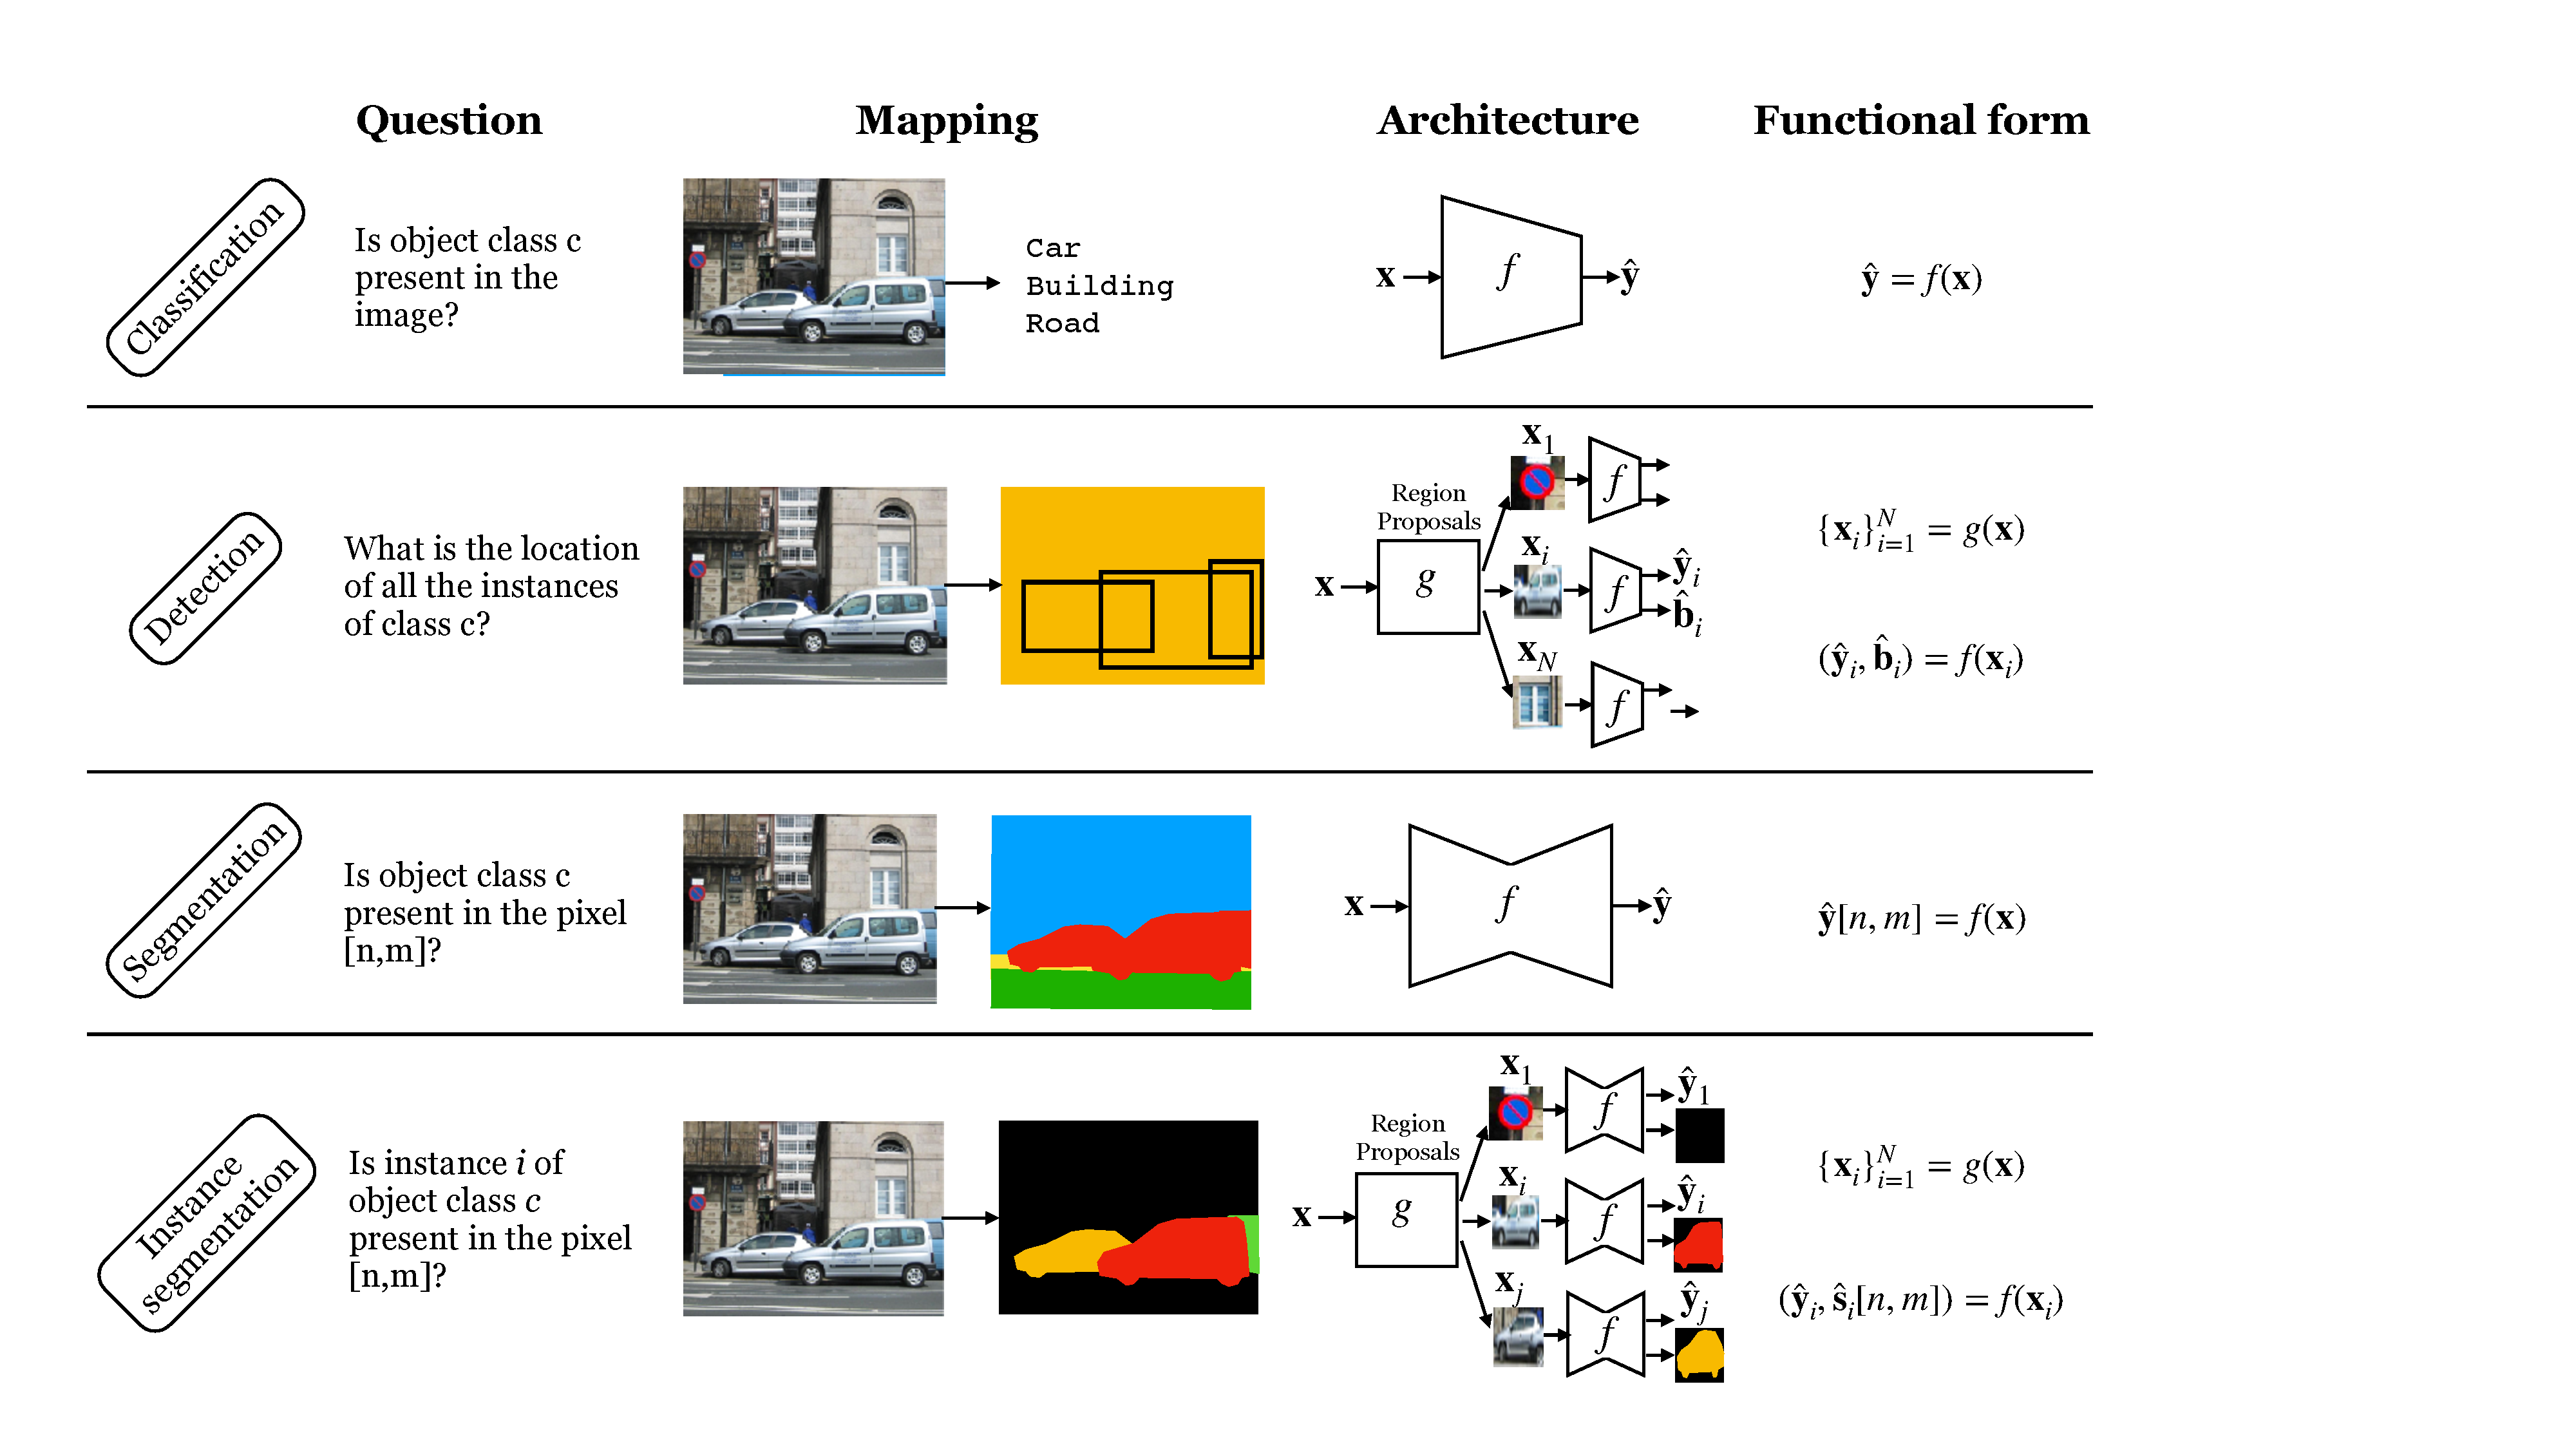
\includegraphics[width=1\linewidth]{figures/object_recognition/model_cards_v2.pdf}
\caption{A family of object recognition definitions.}
\label{fig:pictorialsummary}
\end{figure}

However, the representations we have described in this chapter feel very incomplete. If you are building a robot or an autonomous vehicle, such object representations are very hard to act on. A robot planning to grasp an object will need an accurate three-dimensional (3D) modeling of the object as well as an understanding of some of its physical properties in order to plan for the best grasping points. An autonomous vehicle will also need an accurate 3D description of the locations of objects in the world, together with a characterization of their dynamics. Therefore, object segmentation and classification only provide one part of the information needed.

%\reviewcomment{There are two follow up chapters missing: one on theories on object recognition where we cover fundamentals such as categorization theories, objects in context, what is an object, related tasks such as material recognition, ... And one chapter on scene level understanding with 3d objects.}


% \begin{comment}

% \section{Layers}

% the segmentation feels also a bit incomplete as it treats the output as a 2D image. But when we look at a scene, we also have labels for things that are occluded.

% - handling multiple instances and occlusion
% - a modal object completion

% When formulated as a learning problem, the trick is to specify an output data structure that is learnable and satisfies our requirements. One example is, we could specify a label and output a binary segmentation mask and z ordering value.

% $(s,z) = f(x,y)$

% but then what happens if we have 

% or w
% \section{3D}
% - meshes
% - point clouds
% - voxels
% - volumetric models









% % -> what is in forsyth book?

	
		
		
% 	Models
% 		blocks world
% 		3d compositional models
% 		geons
% 		deformable parts
% 		pictorial structures
% 		scene models
% 		context

		

			
% 	Similarity based models
% 		Prototypes
% 		Attributes
% 		Retrieval, similarity measures
% 		Retrieval by deformable alignment. 
		
% 	Semantic segmentation 
% 		Pixel classification: what is the generic formulation? 
	
	
	
% 	Levels of supervision - this go in another chapter? or maybe something very specific about this chapter. 
		
		
% 	Technical tricks
% 		Hard negative mining
% 		Non-maximal  supression

% 	Challenges
% 		Learning from little data
% 		Unsupervised object discovery
		
% 	Beyond recognition
% 		Attributes and affordances
% 		Shape base representations (deformable fields)
% 		Open world
		
% %\chapter{3D scene understanding}


% \end{comment}